\documentclass{article}
\usepackage{authblk}
\usepackage{amsfonts}
\usepackage{amsmath}
\usepackage[english]{babel}
\usepackage{blindtext}
\usepackage{cancel}
\usepackage{caption}
\usepackage{colortbl}
\usepackage[utf8]{inputenc}
\usepackage{csquotes}
\usepackage[T1]{fontenc}
\usepackage{float}
\usepackage[a4paper]{geometry}
\usepackage{graphicx}
\usepackage{listings}
\usepackage{lipsum}
\usepackage{lmodern}
\usepackage{mathrsfs}
\usepackage{physics}
\usepackage{scrextend}
\usepackage{simplewick}
\usepackage{slashed}
\usepackage{stackengine}
\usepackage{subcaption}
\usepackage{tikz}
\usepackage[compat=1.1.0]{tikz-feynman}
\usepackage{yhmath}

\newcommand{\parcial}[2]{\frac{\partial #1}{\partial #2}}
\newcommand{\dtotal}[2]{\frac{d#1}{d#2}}
\newcommand{\s}[1]{\slashed #1}
\newcommand{\lag}{\mathscr{L}}
\restylefloat{figure}
\renewcommand{\baselinestretch}{1.1}
\DeclareMathOperator{\erfi}{erfi}
% \numberwithin{equation}{section}
%\renewcommand\thesection{Exercise \arabic{section}}
% \renewcommand\thesubsection{\Roman{subsection}.}


\title{Bremsstrahlung}
\author{PROVAPROVA}

% \setlength{\textwidth}{155mm}
% \setlength{\textheight}{195mm}
% \setlength{\oddsidemargin}{6mm}
% \setlength{\evensidemargin}{28mm}
% \setlength{\topmargin}{-5mm}
\geometry{top=2cm, bottom=2.0cm, left=2cm, right=2cm}

\begin{document}

\maketitle

We want to compute the Bremsstrahlung contribution
in the limit of soft emitted photons for a given process $N \to M$,
where $N$ particles scatter into $M$ particles.

\begin{center}
	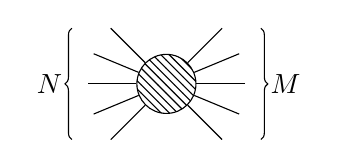
\begin{tikzpicture}
	\begin{feynman}
	\vertex[blob] (m) at ( 0, 0) {};
	\vertex (a) at (1.2,-0.707);
	\vertex (a1) at (0.707,-0.707);
	\vertex (a2) at (0.924,-0.383);
	\vertex (a3) at (1,0);
	\vertex (a4) at (0.924,0.383);
	\vertex (a5) at (0.707,0.707);
	\vertex (b) at (1.2,0.707);
	\vertex (c) at (-1.2,0.707);
	\vertex (b1) at (-0.707,0.707);
	\vertex (b2) at (-0.924,0.383);
	\vertex (b3) at (-1,0);
	\vertex (b4) at (-0.924,-0.383);
	\vertex (b5) at (-0.707,-0.707);
	\vertex (d) at (-1.2,-0.707);
	\diagram* {
		(a1) -- (m) -- (b1),
		(a2) -- (m) -- (b2),
		(a3) -- (m) -- (b3),
		(a4) -- (m) -- (b4),
		(a5) -- (m) -- (b5),
	};
	\end{feynman}
	\draw[decoration={brace}, decorate]
		(d.south west)-- (c.north west)node[pos=0.5, left] {  \(N\)};
	\draw[decoration={brace}, decorate]
		(b.north east)-- (a.south east)node[pos=0.5, right] {  \(M\)};
	\end{tikzpicture}
\end{center}

Let's assume that we know the amplitude for this process.
We will denote this amplitude by $\mathcal{H}(p)$,
where $p = \{p_1, p_2, \ldots, p_N, p_{N+1}, \ldots, p_{N+M}\}$.
With $p_i$ the initial 4-momenta if $i\leq N$, and the final 4-momenta if $N<i\leq N+M$.
Of course, 4-momentum conservation tells us that
\begin{equation*}
	\sum_{i=1}^{N}p_i - \sum_{i=N+1}^{N+M} p_i
	= \sum_i \xi_i p_i
	= 0
\end{equation*}
Where we define $\xi=1$ for initial particles ($0<i\leq N$)
and $\xi=-1$ for final particles ($N<i\leq N+M$);
\begin{equation*}
    \xi
    = \begin{cases}
        +1 & \text{initial particles}\\
        -1 & \text{final particles}\\
    \end{cases}
\end{equation*}

Also, we will use the following notation;
consider the whole amplitude except for the Feynman rule
associated with some external line $k$
(that is, the amplitude $\mathcal{H}$ with the $k$th leg amputated),
if the amputated leg corresponds to an initial fermion or a final anti-fermion
we will denote such amplitude by $\bar{\mathcal{H}}_k(p)$.
If it corresponds to an initial anti-fermion or a final fermion,
then we will denote it by $\mathcal{H}_k(p)$.
Note then that we have the following 4 cases for initial/final (anti-)fermions:
\begin{equation}\label{eq:Hard_amplitude_definition}
	\mathcal{H}(p)
	= \begin{cases}
		\bar{v}(p_k)\mathcal{H}_k(p) & \text{ for an initial anti-fermion}\\
		\bar{\mathcal{H}}_k(p)u(p_k) & \text{ for an initial fermion}\\
		\bar{\mathcal{H}}_k(p)v(p_k) & \text{ for a final anti-fermion}\\
		\bar{u}(p_k)\mathcal{H}_k(p) & \text{ for a final fermion}
	\end{cases}
\end{equation}

\section{Leading Power}
\begin{center}
	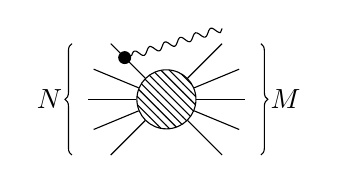
\begin{tikzpicture}
	\begin{feynman}
	\vertex[blob] (m) at ( 0, 0) {};
	\vertex (a) at (1.2,-0.707);
	\vertex[dot] (gi) at (-0.530,0.530) {};
	\vertex (gf) at (0.707,0.9);
	\vertex (a1) at (0.707,-0.707);
	\vertex (a2) at (0.924,-0.383);
	\vertex (a3) at (1,0);
	\vertex (a4) at (0.924,0.383);
	\vertex (a5) at (0.707,0.707);
	\vertex (b) at (1.2,0.707);
	\vertex (c) at (-1.2,0.707);
	\vertex (b1) at (-0.707,0.707);
	\vertex (b2) at (-0.924,0.383);
	\vertex (b3) at (-1,0);
	\vertex (b4) at (-0.924,-0.383);
	\vertex (b5) at (-0.707,-0.707);
	\vertex (d) at (-1.2,-0.707);
	\diagram* {
		(a1) -- (m) -- (b1),
		(a2) -- (m) -- (b2),
		(a3) -- (m) -- (b3),
		(a4) -- (m) -- (b4),
		(a5) -- (m) -- (b5),
		(gi) --[photon] (gf),
	};
	\end{feynman}
	\draw[decoration={brace}, decorate]
		(d.south west)-- (c.north west)node[pos=0.5, left] {  \(N\)};
	\draw[decoration={brace}, decorate]
		(b.north east)-- (a.south east)node[pos=0.5, right] {  \(M\)};
	\end{tikzpicture}
\end{center}
Consider now that we emit a photon from one of the external legs of the diagram.
For example, let's focus on the case of an initial anti-fermion.
If the momentum of this particle is $p_k$
(with $k\leq N$ in this case, since it is an initial particle),
and the momentum of the photon is $k$ we can compute the amplitude as
\begin{equation}\label{Amplitude}
	\mathcal{A}
	= \varepsilon^*_\mu(k) \bar{v}(p_k) (-iQ \gamma^\mu)
	\frac{i(\s{k} - \s{p}_k + m)}{(p_k - k)^2 - m^2}
	\mathcal{H}_k(p_1, \ldots, p_k-k, \ldots, p_{N+M})
\end{equation}
where $\mathcal{H}_k$ is the amputated amplitude defined in
\eqref{eq:Hard_amplitude_definition}.
Because we are interested in soft photons,
we can do the limit $k\to 0$ so that the leading amplitude is
\begin{equation}
	\mathcal{A}
	= Q \varepsilon^*_\mu(k) \bar{v}(p_k) \gamma^\mu
	\frac{-\s{p}_k + m + \order{k}}{-2p_k \cdot k}
	\left[\mathcal{H}_k(p) + \order{k}\right]
	= Q \varepsilon^*_\mu(k) \bar{v}(p_k)
	\frac{-\gamma^\mu\s{p}_k + m\gamma^\mu}{-2p_k \cdot k} \mathcal{H}_k(p)
	+ \order{1}
\end{equation}
where we have used $p_k^2=m^2$ and $k^2=0$ because they are on-shell particles.
Using also the gamma properties
$\gamma^\mu \gamma^\nu = 2 g^{\mu\nu}-\gamma^\nu \gamma^\mu$
and Dirac's equation $\bar{v}(\s{p}+m) = 0$ we obtain
\begin{align*}
	\mathcal{A} &
	= Q \varepsilon^*_\mu(k) \bar{v}(p_k)
	\frac{-2p_k^\mu + (\s{p}_k + m)\gamma^\mu}{-2p_k\cdot k} \mathcal{H}_k(p)
	+ \order{1}
	= Q \frac{\varepsilon^*(k) \cdot p_k}{p_k \cdot k} \bar{v}(p_k) \mathcal{H}_k(p)
	+ \order{1}\\&
	= Q \frac{\varepsilon^*(k) \cdot p_k}{p_k \cdot k} \mathcal{H}(p)
	+ \order{1}
\end{align*}
So, the emission of a soft-photon, to leading power expansion (LP)
is just the multiplication of the previous amplitude $\mathcal{H}$ by a factor
\footnote{
	Note that $Q$ follows from the vertex factor,
	and therefore is always the charge associated with the field,
	so the charge of a fermion and anti-fermion is the same.
}
$Q \frac{\varepsilon^*(k) \cdot p_k}{p_k \cdot k}$.

One can repeat the same argument,
with the other 3 cases and the result is always the same,
except for a overall sign, we can summarize all the cases by writing:
\begin{equation*}
	\mathcal{A}^{LP}
	= \eta Q \frac{\varepsilon^*(k) \cdot p_k}{p_k \cdot k} \mathcal{H}(p)
\end{equation*}
with
\begin{equation}\label{eq:definition eta}
	\eta
	= \begin{cases}
        \xi & \text{ for anti-fermions}\\
        -\xi & \text{ for fermions}\\
    \end{cases}
    = \begin{cases}
		1 & \text{ for initial anti-fermions and final fermions}\\
		-1 & \text{ for final anti-fermions and initial fermions}\\
	\end{cases}
\end{equation}
Alternatively, one could just absorb a $-$ sign on both $\eta$ and $Q$,
only for anti-fermions.
In such a case, now $Q$ would be the charge of the particle,
not the charge of the field
(so that anti-fermions and fermions would have opposite charge)
and then $\eta$ would be -1 for all initial particles and 1 for all final particles.
Since the product $\eta Q$ is not affected by this,
both definitions for $\eta$ and $Q$ are equally valid,
as long as the same convention is used consistently everywhere.

%Thanks to this factorization, we can write these amplitudes using a new kind of Feynman rule, which we will call the eikonal Feynman rule, written as
%
%\begin{equation}
%	\feynmandiagram[inline=(d.base),horizontal=d to b] {
%		a -- [double] b -- [double] c,
%		b -- [boson] d,
%	};
%	= \eta Q \frac{p^\mu_k}{p_k \cdot k}
%\end{equation}
%Then, we can write the amplitude diagrammatically as
%\begin{center}
%	\begin{tikzpicture}
%	\begin{feynman}
%	\vertex[blob] (m) at ( 0, 0) {};
%	\vertex (v2) at (-2, -0.5);
%	\vertex (a) at (1.2,-0.707);
%	\vertex (gi) at (-2.5,-0.5);
%	\vertex (gf) at (-1.5,-0.5);
%	\vertex (e) at (-2, 0.5);
%	\vertex (a1) at (0.707,-0.707);
%	\vertex (a2) at (0.924,-0.383);
%	\vertex (a3) at (1,0);
%	\vertex (a4) at (0.924,0.383);
%	\vertex (a5) at (0.707,0.707);
%	\vertex (b) at (1.2,0.707);
%	\vertex (c) at (-1.2,0.707);
%	\vertex (b1) at (-0.707,0.707);
%	\vertex (b2) at (-0.924,0.383);
%	\vertex (b3) at (-1,0);
%	\vertex (b4) at (-0.924,-0.383);
%	\vertex (b5) at (-0.707,-0.707);
%	\vertex (d) at (-1.2,-0.707);
%	\diagram* {
%		(a1) -- (m) -- (b1),
%		(a2) -- (m) -- (b2),
%		(a3) -- (m) -- (b3),
%		(a4) -- (m) -- (b4),
%		(a5) -- (m) -- (b5),
%		(gi) --[double] (v2) --[double] (gf),
%		(v2) --[photon] (e),
%	};
%	\end{feynman}
%	\end{tikzpicture}
%\end{center}

We can now compute the amplitude for soft Bremsstrahlung; $N \to M + \gamma$.
Since the photon can be emitted from different particles,
we must sum over all the possible external legs, and the result is
\begin{equation}\label{ALP}
	\mathcal{A}^{LP}
	= \sum_i \eta_i Q_i \frac{\varepsilon^*(k) \cdot p_i}{p_i \cdot k} \mathcal{H}(p)
\end{equation}
the fact that neutral particles cannot emit a photon
is already taken into account because every term is proportional to $Q_i$.
Actually, there could also be a photon being emitted from the internal propagators,
so we should also sum over all the possible photons emitted by internal lines.
Let's see that such terms are already of order $\order{1}$, so we can ignore them at LP.

Indeed, if the photon is emitted from one propagator with momentum $\bar{p}$,
we can always write the elastic amplitude as
\begin{equation}
	\mathcal{H}(p)
	= \overline{\mathcal{H}}_L(p, \bar{p})
	\frac{i(\bar{\s{p}} + m)}{\bar{p}^2 - m^2} \mathcal{H}_R(p, \bar{p})
\end{equation}
And then, the amplitude with the emitted photon will be
\begin{align*}
	\mathcal{A} &
	= \varepsilon^*_\mu(k) \overline{\mathcal{H}}_L(p, \bar{p})
	\frac{i(\bar{\s{p}} + m)}{\bar{p}^2 - m^2} (-i Q \gamma^\mu)
	\frac{i(\bar{\s{p}} + \s{k} + m)}{(\bar{p} + k)^2 - m^2}
	\mathcal{H}_R(p, \bar{p}+k)\\&
	= Q \varepsilon^*_\mu(k) \overline{\mathcal{H}}_L(p, \bar{p})
	\frac{\bar{\s{p}} + m}{\bar{p}^2 - m^2} \gamma^\mu
	\frac{i(\bar{\s{p}} + m)}{\bar{p}^2 - m^2} \mathcal{H}_R(p, \bar{p})
	+ \order{k}
	= \order{1}
\end{align*}
So, it is clear that the key factor is the denominator $(p \pm k)^2 - m^2$.
If $p^2 = m^2$, this factor is of order $\order{k}$
and reduces the order of the whole expression by 1.
But, if $p^2\neq m^2$, then it is of order $\order{1}$
and it doesn't reduce the order of the overall expression,
so photons emitted from real particles contribute one order of magnitude more
than photons emitted by internal lines.

In general, one probably wants to compute cross-sections, to compare with experiments.
To do it, we need to compute the amplitude squared
(and we will average over polarizations).
\\
Because the amplitude factorizes we can compute the square immediately,
using equation \eqref{ALP}
\begin{equation}\label{A2LP}
	\overline{|\mathcal{A}^{LP}|}^2
	= - \sum_{i, j} \eta_i \eta_j Q_i Q_j
	\frac{p_i \cdot p_j}{(p_i \cdot k)(p_j \cdot k)}
	\overline{|\mathcal{H}|}^2
\end{equation}
where we have used the sum over polarizations
$\sum \varepsilon_\mu^* \varepsilon_\nu = -g_{\mu \nu}$,
there are other contributions to this relation that are
proportional to $k$ in the polarization sum.
Those contributions can be neglected at leading power,
but they must vanish anyway due to the Ward identity ($k_\mu \mathcal{A}^\mu = 0$).

\section{Next to Leading Power}
We have seen that the LP term of a photon emission can be computed
easily given the amplitude of the non-radiative process, $\mathcal{H}$.
Now, we can look into the Next-to-Leading Power (NLP) contribution to the amplitude.
If we focus on the case where the photon is emitted by an outgoing anti-fermion
the amplitude will be given by
\begin{align}\label{eq:A_NLP outgoing anti-fermion}
	\mathcal{A} &
	= \varepsilon^*_\mu(k)
	\bar{\mathcal{H}}_j(p_1, \ldots, p_j+k, \ldots, p_{N+M})
	\frac{i(-\s{k} - \s{p}_j + m)}{(p_j + k)^2 - m^2} (-iQ \gamma^\mu) v(p_j)\nonumber\\&
	= - Q \varepsilon^*_\mu(k)
	\left[\bar{\mathcal{H}}_j(p) + k^\nu \pdv{\bar{\mathcal{H}}_k(p)}{p_j^\nu}\right]
	\frac{\s{k}\gamma^\mu + 2p_j^\mu}{2k \cdot p_j} v(p_j)
	+ \order{k}\nonumber\\&
	= - Q \varepsilon^*_\mu(k)
	\left[\bar{\mathcal{H}}_j(p) + k^\nu \pdv{\bar{\mathcal{H}}_j(p)}{p_j^\nu}\right]
	\frac{2p_j^\mu + k^\mu + i k_\nu \sigma^{\mu\nu}}{2k \cdot p_j} v(p_j)
	+ \order{k}\nonumber\\&
	= \frac{- Q \varepsilon^*_\mu(k)}{2k \cdot p_j}
	\left[
		(2p_j + k)^\mu \mathcal{H}
		+ i k_\nu \bar{\mathcal{H}}_j(p) \sigma^{\mu\nu} v(p_j)
		+ 2p_j^\mu k^\nu \pdv{\bar{\mathcal{H}}_j(p)}{p_j^\nu} v(p_j)
	\right]
	+ \order{k}
\end{align}
Where we have used that $\s{k}\gamma^\mu = k^\mu + i k_\nu \sigma^{\mu\nu}$
with $\sigma^{\mu\nu} = \frac{i}{2}\comm{\gamma^\mu}{\gamma^\nu}$.
We can see that the first term corresponds exactly to the LP amplitude
(with an extra contribution proportional to $k^\mu$).
But in the other two terms, we cannot obtain the elastic amplitude $\mathcal{H}$,
so there is no obvious factorization at NLP.
The general formula for the photon emitted on incoming/outgoing external legs
for particle/anti-particle is

\begin{equation*}
	\mathcal{A}
	= \frac{\eta_j Q \varepsilon^*_\mu(k)}{2k \cdot p_j}
	\left[
		(2p_j - \xi_j k)^\mu \mathcal{H}
		+ i\eta_j\xi_j k_\nu \hat{\sigma}_j^{\mu\nu}\mathcal{H}
		- 2\xi_j p_j^\mu k^\nu \hat{D}_{j\nu}\mathcal{H}
	\right]
	+ \order{k}
\end{equation*}
where, as before, $\xi$ is $-1$ for outgoing particles and $1$ for incoming
and $\eta$ is defined in equation \eqref{eq:definition eta}.
The terms $\hat{\sigma}_j^{\mu\nu}\mathcal{H}$ and $\hat{D}_{j\nu}\mathcal{H}$
are operators acting on the amplitude,
the definition of those operators should be clear from
equation \eqref{eq:A_NLP outgoing anti-fermion}:
$\hat{\sigma}_j^{\mu\nu}\mathcal{H}$ gives the amplitude $\mathcal{H}$
inserting a $\sigma^{\mu\nu}$ in the $j$th external leg.
On the other hand $\hat{D}_{j\nu}\mathcal{H}$ is defined by taking the derivative of the amputated amplitude with respect to $p^\nu_j$, and inserting the legs back afterwards.

To get the total amplitude for Bremsstrahlung,
we need to sum over all possible legs emitting the photon.
But now, since we are interested in keeping $\order{1}$ terms,
we can no longer neglect the photons emitted from internal legs.
The total amplitude therefore will have the form
\begin{equation}
	\mathcal{A}
	= \varepsilon^*_\mu (\mathcal{A}^\mu_{\mathrm{ext}}
	+ \mathcal{A}^\mu_{\mathrm{int}})
\end{equation}
The external part is easy to compute, is just the sum over all external legs:
\begin{equation}\label{A_ext}
	\mathcal{A}^\mu_{\mathrm{ext}}
	= \sum_i\frac{\eta_i Q_i}{2k\cdot p_i}
	\left[
		(2p_i - \xi_i k)^\mu
		+ i\eta_i\xi_i k_\nu \hat{\sigma}_i^{\mu\nu}
		- 2\xi_i p_i^\mu k^\nu \hat{D}_{i\nu}
	\right] \mathcal{H}
	+ \order{k}
\end{equation}
Now, the Ward identity can be used to obtain the relation
\begin{align*}
	k_\mu \mathcal{A}^\mu_{\mathrm{int}} &
	= -k_\mu \mathcal{A}^\mu_{\mathrm{ext}}
	= -\sum_i \eta_i Q_i
	\left[1 - \xi_i k^\nu \hat{D}_{i\nu}\right] \mathcal{H}
	+\order{k}\\&
	= -\left(\sum_i \eta_i Q_i\right)\mathcal{H}
	+ k_\mu \sum_i \eta_i \xi_i Q_i \hat{D}^\mu_{i}\mathcal{H}
	+ \order{k}
\end{align*}
The first term vanish due to charge conservation, so we can write
\begin{equation}\label{int_amplitude}
	\mathcal{A}^\mu_{\mathrm{int}}
	= \sum_i \eta_i \xi_i Q_i \hat{D}^\mu_{i}\mathcal{H} + K^\mu
	+ \order{k}
\end{equation}
with $K^\mu$ a vector orthogonal to $k$ (i.e. $k \cdot K=0$).
To fulfil this relation this must be proportional either to
$(x\cdot k) k^\mu - k^2 x^\mu$ with an arbitrary vector
$x^\mu$ or to $k_\mu A^{\mu\nu}$ with $A^{\mu\nu}$ an antisymmetric rank-2 tensor.
Both cases are of order $\order{k}$,
so we would need to multiply this factors by terms that behave,
at least, as $1/k$. Such terms only appear from radiation due to external lines,
so are already included in \eqref{A_ext}. So we have that
\begin{equation*}
	K^\mu
	= 0 + \order{k}
\end{equation*}
Combining equation \eqref{int_amplitude} (with $K=0$)
with equation \eqref{A_ext} we obtain
\begin{align*}
	\mathcal{A}^\mu &
	= \sum_i \frac{\eta_i Q_i}{2k \cdot p_i}
	\left[
		(2p_i - \xi_i k)^\mu \mathcal{H}
		+ i\eta_i \xi_i k_\nu \sigma^{\mu\nu}\mathcal{H}
		+ 2\xi_i (k \cdot p_i)
		\left(
			\pdv{\mathcal{H}}{p_{i\mu}}
			- \frac{p_i^\mu k^\nu}{p_i \cdot k} \pdv{\mathcal{H}}{p_i^\nu}
		\right)
	\right]
	+ \order{k}\\&
	= \sum_i \frac{\eta_i Q_i}{2k \cdot p_i}
	\left[
		(2p_i - \xi_i k)^\mu \mathcal{H}
		+ i\eta_i \xi_i k_\nu \sigma^{\mu\nu}\mathcal{H}
		+ 2\xi_i (k \cdot p_i)
		\left(g^{\mu\nu} - \frac{p_i^\mu k^\nu}{p_i \cdot k}\right)
		\pdv{\mathcal{H}}{p_{i}^\nu}
	\right]
	+ \order{k}
\end{align*}
If we define the tensor
\begin{equation}
	G_i^{\mu\nu}
	= g^{\mu\nu} - \frac{p_i^\mu k^\nu}{p_i\cdot k}
\end{equation}
Then we can write the amplitude as
\begin{equation}\label{ANLP}
	\mathcal{A}^\mu
	= \sum_i \frac{\eta_i Q_i}{2k \cdot p_i}
	\left[
		(2p_i - \xi_i k)^\mu \mathcal{H}
		+ i\eta_i \xi_i k_\nu \sigma^{\mu\nu} \mathcal{H}
		+ 2\xi_i (k \cdot p_i) G_i^{\mu \nu} \pdv{\mathcal{H}}{p_{i}^\nu}
	\right]
	+ \order{k}
\end{equation}
\\
Another way of writing this amplitude is
\begin{align*}
	\mathcal{A}^\mu &
	= \sum_i \frac{\eta_i Q_i}{2k \cdot p_i}
	\left[
		(2p_i - \xi_i k)^\mu \mathcal{H}
		+ i\eta_i \xi_i k_\nu \sigma^{\mu\nu} \mathcal{H}
		+ 2\xi_i
		\left(
			k \cdot p_i \pdv{\mathcal{H}}{p_{i\mu}}
			- p_i^\mu k^\nu \pdv{\mathcal{H}}{p_i^\nu}
		\right)
	\right]
	+ \order{k}\\&
	= \sum_i \frac{\eta_i Q_i}{2k \cdot p_i}
	\left[
		(2p_i - \xi_i k)^\mu \mathcal{H}
		+ i\eta_i \xi_i k_\nu \sigma^{\mu\nu} \mathcal{H}
		+ 2\xi_i k_\nu
		\left(
			p^\nu_i \pdv{\mathcal{H}}{p_{i\mu}} - p_i^\mu \pdv{\mathcal{H}}{p_{i\nu}}
		\right)
	\right]+\order{k}
\end{align*}
Because in the momentum representation, the $\hat{p}$ operator is just multiply by $p$,
and the $\hat{x}$ operator is $i\pdv{p}$ (such that $[\hat{x}, \hat{p}]=1$)
we can rewrite the last term in parenthesis as
\begin{equation}
	\hat{p}^\nu_i(-i\hat{x}^\mu_i) \mathcal{H}
	- \hat{p}^\mu_i (-i\hat{x}^\nu_i) \mathcal{H}
	= -i\left(\hat{p}^\nu_i \hat{x}^\mu_i - \hat{p}^\mu_i \hat{x}^\nu_i\right)
	\mathcal{H}
	= -i\left(\hat{x}^\mu_i \hat{p}^\nu_i - 1 - \hat{x}^\nu_i \hat{p}^\mu_i + 1\right)
	\mathcal{H}
	= -i\hat{L}^{\mu\nu} \mathcal{H}
\end{equation}
On the other hand, for spin $\frac{1}{2}$ the spin operator is given by
$\Sigma^{\mu\nu}=\frac{1}{2}\sigma^{\mu\nu}$.
So, the middle term is the contribution of spin,
while the third term is the contribution of the orbital angular momentum.

Now, as before we may want to compute the squared amplitude,
since it's the one we need to integrate to obtain physical predictions.
Of course, because we have the amplitude written as
$$\mathcal{A}=\mathcal{A}^{LP} + \mathcal{A}^{NLP} + \order{k}$$
the squared amplitude will be of the form
\begin{equation}
	|\mathcal{A}|^2
	= |\mathcal{A}^{LP}|^2 + \mathcal{A}^{*LP}\mathcal{A}^{NLP}
	+ \mathcal{A}^{LP}\mathcal{A}^{*NLP}
	+ \order{1}
\end{equation}
Note that $\mathcal{A}^{LP} \order{k} = \order{1}$,
so we need to neglect any term of $ \order{1}$ if we want to be consistent.
The two terms we need to compute are:
\begin{equation}
	\mathcal{A}^{*LP} \mathcal{A}^{NLP}
	= \sum_{i,j} \frac{-\eta_i \eta_j Q_i Q_j p_{i\mu}}{2(k \cdot p_i)(k \cdot p_j)}
	\mathcal{H}^*
	\left[
		- \xi_j k^\mu \mathcal{H}
		+ i\eta_j \xi_j k_\nu \sigma^{\mu\nu} \mathcal{H}
		+ 2\xi_j (k \cdot p_j) G_j^{\mu \nu} \pdv{\mathcal{H}}{p_{j}^\nu}
	\right]
\end{equation}
The first term in the sum vanishes due to charge conservation because
\begin{equation}
	\sum_{i,j}
	\frac{\eta_i \eta_j\xi_j Q_i Q_j (p_{i} \cdot k)}{2(k \cdot p_i)(k \cdot p_j)}
	\mathcal{H}^* \mathcal{H}
	= \sum_{j} \frac{\eta_j \xi_j Q_j}{2(k \cdot p_j)} \left(\sum_i \eta_i Q_i\right)
	\mathcal{H}^* \mathcal{H}
\end{equation}
and the sum over $i$ vanishes. The same cancellation occurs in
$\mathcal{A}^{LP}\mathcal{A}^{*NLP}$ leaving with only
\begin{equation*}
	\mathcal{A}^{LP} \mathcal{A}^{*NLP}
	= \sum_{i,j} \frac{-\eta_i \eta_j Q_i Q_j p_{i\mu}}{2(k \cdot p_i)(k \cdot p_j)}
	\left[
		i\eta_j \xi_j k_\nu \sigma^{\mu\nu} \mathcal{H}
		+ 2\xi_j (k \cdot p_j) G_j^{\mu \nu} \pdv{\mathcal{H}}{p_{j}^\nu}
	\right]^* \mathcal{H}
\end{equation*}
Adding these two terms we are left with the expression
\begin{equation}\label{2Re}
	2\Re{\mathcal{A}^{*LP} \mathcal{A}^{NLP}}
	= \sum_{i,j} \frac{-\eta_i \eta_j Q_i Q_j p_{i\mu}}{2(k \cdot p_i)(k \cdot p_j)}
	2\Re{
		\mathcal{H}^*
		\left[
			i\eta_j \xi_j k_\nu \sigma^{\mu\nu} \mathcal{H}
			+ 2\xi_j (k \cdot p_j) G_j^{\mu \nu} \pdv{\mathcal{H}}{p_{j}^\nu}
		\right]
	}
\end{equation}
Let's see how we can simplify the term in curly brackets
\begin{equation*}
	\mathcal{H}^*
	\left[
		i\eta_j \xi_j k_\nu \sigma^{\mu\nu}\mathcal{H}
		+ 2\xi_j (k \cdot p_j) G_j^{\mu \nu} \pdv{\mathcal{H}}{p_{j}^\nu}
	\right]
	+ \left[
		i\eta_j \xi_j k_\nu \sigma^{\mu\nu} \mathcal{H}
		+ 2\xi_j (k \cdot p_j) G_j^{\mu \nu} \pdv{\mathcal{H}}{p_{j}^\nu}
	\right]^*
	\mathcal{H}
\end{equation*}
Let's assume that particle $j$ is a fermion in the final state,
then $\mathcal{H}=\bar{u}(p_j) \mathcal{H}_j(p)$, $\eta_j=1$, $\xi_j=-1$.
Using the properties $\bar{u}^\dag = \gamma^0u$,
$\sigma_{\mu\nu}^\dag = \gamma^0 \sigma_{\mu\nu}\gamma^0$ we can write it like
\begin{equation*}
	-\mathcal{H}_j^\dag \gamma^0 u_j \left[
		i k_\nu \bar{u}_j \sigma^{\mu\nu} \mathcal{H}_j
		+2 (k \cdot p_j) G_j^{\mu \nu} \bar{u}_j \pdv{\mathcal{H}_j}{p_{j}^\nu}
	\right]
	- \left[
		- i k_\nu \mathcal{H}_j^\dag \gamma^0 \sigma^{\mu\nu} u_j
		+ 2(k \cdot p_j) G_j^{\mu \nu} \pdv{\mathcal{H}^\dag_j}{p_{j}^\nu} \gamma^0 u_j
	\right] \bar{u}_j \mathcal{H}_j
\end{equation*}
\begin{equation*}
	-i k_\nu \mathcal{H}_j^\dag \gamma^0 u_j \bar{u}_j \sigma^{\mu\nu} \mathcal{H}_j
	- 2 (k \cdot p_j) G_j^{\mu \nu} \mathcal{H}_j^\dag \gamma^0 u_j
	\bar{u}_j \pdv{\mathcal{H}_j}{p_{j}^\nu}
	+ i k_\nu \mathcal{H}_j^\dag \gamma^0 \sigma^{\mu\nu} u_j \bar{u}_j \mathcal{H}_j
	- 2(k \cdot p_j) G_j^{\mu \nu} \pdv{\mathcal{H}^\dag_j}{p_{j}^\nu} \gamma^0 u_j
	\bar{u}_j \mathcal{H}_j
\end{equation*}
If we sum over all the possible polarizations of $j$ we can write $u\bar{u}\to \s{p}+m$
\begin{equation*}
	i k_\nu \mathcal{H}_j^\dag \gamma^0
	\left(\sigma^{\mu\nu}(\s{p}_j + m) - (\s{p}_j + m) \sigma^{\mu\nu}\right) \mathcal{H}_j
	- 2(k \cdot p_j) G_j^{\mu \nu} \mathcal{H}_j^\dag
	\gamma^0 (\s{p}_j + m) \pdv{\mathcal{H}_j}{p_{j}^\nu}
	- 2(k \cdot p_j) G_j^{\mu \nu} \pdv{\mathcal{H}^\dag_j}{p_{j}^\nu}
	\gamma^0 (\s{p}_j + m) \mathcal{H}_j
\end{equation*}
In the first term we need to compute the commutator
\begin{align*}
	ik_\nu \comm{\sigma^{\mu\nu}}{\s{p}_j + m}&
	= i k_\nu p_{j\lambda} \comm{\sigma^{\mu\nu}}{\gamma^\lambda}
	= -2k_\nu p_{j\lambda}
	\left(g^{\lambda \nu} \gamma^\mu - g^{\lambda \mu} \gamma^\nu\right)
	= -2\left((k \cdot p_j) g^{\mu\nu} - k^\nu p_{j}^\mu\right) \gamma_\nu \\&
	= -2(k \cdot p_j) G^{\mu\nu} \gamma_\nu
	= -2(k \cdot p_j) G^{\mu\nu} \pdv{(\s{p}_j + m)}{p_{j}^\nu}
\end{align*}
Combining now all the terms we are left with
\begin{equation*}
	-2(k \cdot p_j) G_j^{\mu \nu} \mathcal{H}_j^\dag \gamma^0
	\pdv{(\s{p}_j + m)}{p_{j}^\nu} \mathcal{H}_j
	- 2(k \cdot p_j) G_j^{\mu \nu} \mathcal{H}_j^\dag \gamma^0
	(\s{p}_j + m) \pdv{\mathcal{H}_j}{p_{j}^\nu}
	- 2(k \cdot p_j) G_j^{\mu \nu} \pdv{\mathcal{H}^\dag_j}{p_{j}^\nu}
	\gamma^0 (\s{p}_j + m) \mathcal{H}_j
\end{equation*}
\begin{equation*}
	-2(k \cdot p_j) G_j^{\mu \nu}
	\pdv{(\mathcal{H}_j^\dag \gamma^0 (\s{p}_j + m)\mathcal{H}_j)}{p_j^\nu}
	= -2(k \cdot p_j) G_j^{\mu \nu} \pdv{\overline{|\mathcal{H}|}^2}{p_j^\nu}
\end{equation*}
Even though we don't have factorization in the amplitude level,
we recover the factorization when squaring the amplitude.
For the other cases, the same argument holds and we obtain
\begin{equation*}
	2\Re{
		\mathcal{H}^* \left[
			i\eta_j \xi_j k_\nu \sigma^{\mu\nu} \mathcal{H}
			+ 2\xi_j (k \cdot p_j) G_j^{\mu\nu} \pdv{\mathcal{H}}{p_{j}^\nu}
		\right]
	}
	= 2\xi_j (k \cdot p_j) G_j^{\mu \nu} \pdv{\overline{|\mathcal{H}|}^2}{p_j^\nu}
\end{equation*}
Substituting now to equation \eqref{2Re}
\begin{equation*}
	2\Re{\overline{\mathcal{A}^{*LP} \mathcal{A}^{NLP}}}
	= -\sum_{i,j} \frac{\eta_i \eta_j \xi_j Q_i Q_j p_{i\mu}}{(k \cdot p_i)}
	G_j^{\mu\nu} \pdv{\overline{|\mathcal{H}|}^2}{p_j^\nu}
\end{equation*}
\\
So the amplitude squared is given by
\begin{equation}
	\overline{|\mathcal{A}|}^2
	= - \sum_{i, j} \eta_i \eta_j Q_i Q_j
	\frac{p_i \cdot p_j}{(p_i \cdot k)(p_j \cdot k)}
	\left[
		1 + \xi_j \frac{(p_j \cdot k) p_{i\mu}}{p_i \cdot p_j} G_j^{\mu\nu} \pdv{p_j^\nu}
	\right]
	\overline{|\mathcal{H}|}^2+ \order{1}
\end{equation}

\subsection{Shifted Kinematics}

This has the inconvenient that one need to compute the derivative of the amplitude $|\mathcal{H}|^2$. Also, the amplitude is evaluated at external momenta $p$, i.e. $|\mathcal{H}(p)|^2$, but because we have the extra photon, conservation of 4-momenta is no longer fulfilled at NLP, i.e. $$\sum_i \xi_i p_i = k \neq 0.$$
To solve this problem we will write the amplitude in a different way, using the fact that derivatives are the generators of translations, i.e. $f(x+a)=f(x)+af'(x)+\order{a^2}$. We want to write the amplitude squared as something like
\begin{equation}
	\overline{|\mathcal{A}|}^2 = A \left[\overline{|\mathcal{H}|}^2 + \sum_j \delta p_j^\nu \pdv{\overline{|\mathcal{H}|}^2}{p_j^\nu}\right]
\end{equation}
where $A$ is just a constant, comparing with our expression, we can define $$A=- \sum_{i, j} \eta_i \eta_j Q_i Q_j \frac{p_i \cdot p_j}{(p_i \cdot k)(p_j \cdot k)}$$but because we need a sum over momenta inside the brackets, we will rewrite the amplitude as follows:
\begin{align*}
	\overline{|\mathcal{A}|}^2 &= A\left[1 - A^{-1}\sum_{i,j} \frac{\eta_i \eta_j\xi_j Q_iQ_j p_{i\mu}}{(k\cdot p_i)} G_j^{\mu\nu}\pdv{p_j^\nu}\right]\overline{|\mathcal{H}|}^2+ \order{1}\\&
	=A\left[1 - \sum_j\left(\eta_j\xi_jQ_j A^{-1}\sum_{i} \frac{\eta_i Q_i p_{i\mu}}{(k\cdot p_i)} G_j^{\mu\nu}\right)\pdv{p_j^\nu}\right]\overline{|\mathcal{H}|}^2+ \order{1}
\end{align*}
so we can identify
\begin{align*}
	\delta p_j^\nu &= \eta_j\xi_jQ_j\left(\sum_{k, l} \eta_k \eta_l Q_k Q_l \frac{p_k \cdot p_l}{(p_k \cdot k)(p_l \cdot k)}\right)^{-1}\sum_{i} \left(\frac{\eta_i Q_i p_{i\mu}}{k\cdot p_i}\right) G_j^{\mu\nu}\\&
	=\eta_j\xi_jQ_j\left(\sum_{k, l} \eta_k \eta_l Q_k Q_l \frac{p_k \cdot p_l}{(p_k \cdot k)(p_l \cdot k)}\right)^{-1}\sum_{i} \left(\frac{\eta_i Q_i}{k\cdot p_i}\right)  \left(p_i^\nu - \frac{p_i\cdot p_j }{p_j\cdot k}k^\nu\right)
\end{align*}
And rewrite the amplitude as
\begin{align}\label{shifted amplitude}
	\overline{|\mathcal{A}|}^2 &=- \sum_{k, l} \eta_k \eta_l Q_k Q_l \frac{p_k \cdot p_l}{(p_k \cdot k)(p_l \cdot k)}\left[1 + \sum_j \delta p_j^\nu \pdv{p_j^\nu}\right]\overline{|\mathcal{H}(p)|}^2+ \order{1}\nonumber\\&
	=- \left(\sum_{i, j} \eta_i \eta_j Q_i Q_j \frac{p_i \cdot p_j}{(p_i \cdot k)(p_j \cdot k)}\right)\overline{|\mathcal{H}(p+\delta p)|}^2+ \order{1}
\end{align}
With this expression we get rid of the derivatives, some properties of $\delta p$ are:
\begin{equation}
	\delta p_j^\nu = \order{k}
\end{equation}
So in the limit $k\to 0$ this vanishes, and we obtain exactly the amplitude \eqref{A2LP}. Another property is
\begin{align*}
	\sum_j \xi_j \delta p_j^\nu&
	= \left(\sum_{k, l} \eta_k \eta_l Q_k Q_l \frac{p_k \cdot p_l}{(p_k \cdot k)(p_l \cdot k)}\right)^{-1}\sum_{i,j} \frac{\eta_jQ_j\eta_i Q_i p_{i\mu}}{k\cdot p_i} G_j^{\mu\nu}\\&
	=\left(\sum_{k, l} \eta_k \eta_l Q_k Q_l \frac{p_k \cdot p_l}{(p_k \cdot k)(p_l \cdot k)}\right)^{-1}\left(\sum_{i} \frac{\eta_i Q_i }{k\cdot p_i} p_i^\nu\sum_j \eta_jQ_j - \sum_{i,j} \frac{\eta_jQ_j\eta_i Q_i }{k\cdot p_i} \frac{p_i \cdot p_j}{p_j\cdot k}k^\nu\right)\\&
	=-\left(\sum_{k, l} \eta_k \eta_l Q_k Q_l \frac{p_k \cdot p_l}{(p_k \cdot k)(p_l \cdot k)}\right)^{-1}\left(\sum_{i,j} \frac{\eta_jQ_j\eta_i Q_i }{k\cdot p_i} \frac{p_i \cdot p_j}{p_j\cdot k}\right)k^\nu
	= -k^\nu
\end{align*}
Where the term with $\sum \eta Q$ vanishes due to charge conservation. This, together with 4-momentum conservation $\sum \xi_j p_j = k$ imply the property
\begin{equation}
	\sum_j \xi_j (p_j + \delta p_j) = k - k= 0
\end{equation}
So the shifted momenta also conserve 4-momenta at LP and NLP, getting rid of the problem we had before.
Finally, we can also see that the shifts are perpendicular to each 4-momentum:
\begin{align*}
	\delta p_j \cdot p_j &= \eta_j\xi_jQ_j\left(\sum_{k, l} \eta_k \eta_l Q_k Q_l \frac{p_k \cdot p_l}{(p_k \cdot k)(p_l \cdot k)}\right)^{-1}\sum_{i} \left(\frac{\eta_i Q_i p_{i\mu}}{k\cdot p_i}\right) G_j^{\mu\nu}p_{j\nu}\\&
	= \eta_j\xi_jQ_j\left(\sum_{k, l} \eta_k \eta_l Q_k Q_l \frac{p_k \cdot p_l}{(p_k \cdot k)(p_l \cdot k)}\right)^{-1}\sum_{i} \left(\frac{\eta_i Q_i}{k\cdot p_i}\right) \left(p_i\cdot p_j - \frac{(p_i\cdot p_j)(p_j\cdot k)}{p_j\cdot k}\right)
	= 0
\end{align*}
Which implies the property
\begin{equation}
	(p+\delta p)^2 = p^2 + 2 p\cdot \delta p + \order{k^2} = m^2 + \order{k^2}
\end{equation}
However, we have the problem that
\begin{align*}
	(\delta p_j)^2 &= Q^2_j\left(\sum_{k, l} \eta_k \eta_l Q_k Q_l \frac{p_k \cdot p_l}{(p_k \cdot k)(p_l \cdot k)}\right)^{-2}\sum_{i,k} \left(\frac{\eta_i Q_i}{k\cdot p_i}\right)\left(\frac{\eta_k Q_k}{k\cdot p_k}\right)  \left(p_i\cdot p_k - \frac{p_k\cdot p_j }{p_j\cdot k}p_i\cdot k - \frac{p_i\cdot p_j }{p_j\cdot k}p_k\cdot k\right)\\&
	=Q^2_j\left(\sum_{k, l} \eta_k \eta_l Q_k Q_l \frac{p_k \cdot p_l}{(p_k \cdot k)(p_l \cdot k)}\right)^{-2}\sum_{i,k} \left(\frac{\eta_i Q_i}{k\cdot p_i}\right)\left(\frac{\eta_k Q_k}{k\cdot p_k}\right)  \left(p_i\cdot p_k\right)\\&
	=Q^2_j\left(\sum_{k, l} \eta_k \eta_l Q_k Q_l \frac{p_k \cdot p_l}{(p_k \cdot k)(p_l \cdot k)}\right)^{-1} \neq 0
\end{align*}
So even if small and negligible at NLP, the masses get shifted by a non-zero amount. This may cause problems if one uses this formalism to do numerical calculations.

For the particular case with only two charged particles; $p_1$ and $p_2$ with $\eta_1Q_1=+1$ and $\eta_2Q_2=-1$
\begin{equation*}
	C = \left(\sum_{k, l} \eta_k \eta_l Q_k Q_l \frac{p_k \cdot p_l}{(p_k \cdot k)(p_l \cdot k)}\right)
	= \frac{m^2_1}{(p_1 \cdot k)^2} -2 \frac{p_1 \cdot p_2}{(p_1 \cdot k)(p_2 \cdot k)}+ \frac{m^2_2}{(p_2 \cdot k)^2}
\end{equation*}
\begin{align*}
	\delta p_1^\nu
	=\left[ \left(\frac{C^{-1}}{k\cdot p_1}\right)  \left(p_1^\nu - \frac{m_1^2}{p_1\cdot k}k^\nu\right) - \left(\frac{C^{-1}}{k\cdot p_2}\right)  \left(p_2^\nu - \frac{p_2\cdot p_1}{p_1\cdot k}k^\nu\right)\right]
\end{align*}


\subsection{Modified Shifted Kinematics}

Would be nice if we could find another expression for $\delta p_i$ in such a way that, in addition to all the previous properties, ensures that masses are not shifted. In other words, we want to find such $\delta p_i$ that
\begin{itemize}
	\item Conserves four-momenta: $\sum_i \xi_i \delta p_i = -k$
	\item Doesn't shift the mass: $(p_i+\delta p_i)^2 = m_i^2$
	\item Still satisfies equation \eqref{shifted amplitude}: $\delta p_j^\nu =\eta_j\xi_jQ_jC^{-1}\sum_{i} \left(\frac{\eta_i Q_i}{k\cdot p_i}\right)  \left(p_i^\nu - \frac{p_i\cdot p_j }{p_j\cdot k}k^\nu\right) + \order{k^2}$
\end{itemize}
\
\\
The most general form that $\delta p_i$ can take is
\begin{equation*}
\delta p_i^\mu = \sum_j A_{ij}^{\mu\nu} p_{j\nu} + B_{i}^{\mu\nu} k_\nu.
\end{equation*}
But is enough for us to consider
\begin{equation*}
\delta p_i^\mu = \sum_j A_{ij} p_{j}^\mu + B_{i} k^\mu.
\end{equation*}
We can restrict to a subset of possible solutions by assuming the set $\{p_i^\mu, k^\mu\}$ to be linearly independent (which is clearly not true in general). This is not a problem since we are only interested in finding a single solution. Furthermore, this assumption allows us to generalize this result even if the shifts can only depend on a restricted subset of external momenta. With this assumption, the conditions to be fulfilled by the coefficients $A$ and $B$ are:
\begin{equation*}
\sum_i \xi_i \delta p_i = -k \Longrightarrow \sum_{i,j} \xi_iA_{ij} p_{j}^\mu + \left(\sum_i \xi_i B_{i}+ 1\right) k^\mu = 0 \Longrightarrow \sum_i \xi_iA_{ij} = 0, \quad \sum_i \xi_iB_{i} =  -1,
\end{equation*}

\begin{align*}
m_i^2 &= (p_i+\delta p_i)^2
= \left(\sum_j \left(\delta_{ij} + A_{ij}\right) p_{j} + B_{i} k\right)^2 \\&
= m_i^2
+\sum_{j,k} \left(2\delta_{ij}A_{ik}+A_{ij}A_{ik}\right)(p_{j}\cdot p_{k})
+2\sum_j \left(\delta_{ij}B_{i}+A_{ij}B_{i}\right)(p_{j}\cdot k).
\end{align*}

Finally, to use this shift for the NLP formula, we need the conditions
\begin{equation*}
A_{ij} = \eta_i\xi_iQ_iC^{-1}\frac{\eta_j Q_j}{k\cdot p_j} + \order{k^2}
\end{equation*}
\begin{equation*}
B_i = -\eta_i\xi_iQ_iC^{-1} \sum_{j} \left(\frac{\eta_j Q_j}{k\cdot p_j}\right)\frac{p_j\cdot p_i }{p_i\cdot k} + \order{k} = - \sum_j A_{ij}\frac{p_i\cdot p_j}{p_i\cdot k} + \order{k}
\end{equation*}
to be satisfied.
\
\\
These conditions are not too restrictive, so we can try to find a solution with the ansatz
\begin{equation*}
A_{ij} = A\eta_i\xi_iQ_i\frac{\eta_j Q_j}{k\cdot p_j}
\end{equation*}
Charge conservation, $\sum_i \eta_i Q_i = 0$, immediately leads to condition $\sum \xi_i A_{ij}=0$ while the other conditions become
\begin{equation}\label{cons_4mom}
\sum_i \xi_i B_i = -1
\end{equation}
\begin{equation}\label{mass_inv}
2A\eta_i\xi_iQ_i\sum_{j}\eta_j Q_j\frac{p_{i}\cdot p_{j}}{k\cdot p_j}+A^2Q^2_iC
+2B_{i}(p_{i}\cdot k)= 0
\end{equation}
\begin{equation*}
A = C^{-1} + \order{k^3}
\end{equation*}
Forcing the mass to be invariant (equation \eqref{mass_inv}) uniquely determines the coefficients $B_i$ as
\begin{equation*}
B_{i}= -A\eta_i\xi_iQ_i\sum_{j}\eta_j Q_j\frac{p_{i}\cdot p_{j}}{(p_{i}\cdot k)(p_j\cdot k)}-\frac{1}{2}\frac{A^2Q^2_iC}{p_i\cdot k}
\end{equation*}
And in the limit $k\to 0$, assuming $A \to C^{-1}=\order{k^2}$, we have
\begin{equation*}
B_{i} \to -\eta_i\xi_iQ_iC^{-1}\sum_{j}\eta_j Q_j\frac{p_{i}\cdot p_{j}}{(p_{i}\cdot k)(p_j\cdot k)}
\end{equation*}
which is the correct behaviour for $B_i$.
Now, we can use the conservation of 4-momentum (equation \eqref{cons_4mom}) to fix the value of $A$. Equation \eqref{cons_4mom} can be written as
\begin{equation*}
1 = -\sum_i \xi_i B_i = A\sum_{i,j} \eta_iQ_i\eta_j Q_j\frac{p_{i}\cdot p_{j}}{(p_{i}\cdot k)(p_j\cdot k)}+\frac{A^2C}{2}\sum_i \frac{\xi_iQ^2_i}{p_i\cdot k} = AC+\frac{A^2C}{2}\sum_i \frac{\xi_iQ^2_i}{p_i\cdot k},
\end{equation*}
which is a quadratic equation. Defining $\chi = \sum_i \frac{\xi_iQ^2_i}{p_i\cdot k}$, we find that the value of $A$ must be
\begin{equation*}
A = \frac{-1}{\chi}\pm \sqrt{\left(\frac{1}{\chi}\right)^2+\frac{2}{C\chi}} = \frac{1}{\chi}\left(-1 \pm \sqrt{1+\frac{2\chi}{C}}\right).
\end{equation*}
Note that $\chi$ is not necessarily positive, so the $\pm$ in the LHS is not the same as the $\pm$ in the RHS. As we will see now, the RHS leads to a more natural formula.
Indeed, in the limit $k \to 0$, we have then
\begin{equation*}
A \to \frac{1}{\chi}\left(-1 \pm \left(1+\frac{\chi}{C}\right)\right)
\end{equation*}
So, the $+$ solution has the correct behaviour at low $k$ and we have found a solution:

\begin{equation}
    \boxed{\delta p_i^\mu = A\eta_i\xi_iQ_i\sum_j \frac{\eta_j Q_j}{k\cdot p_j} p_{j\nu}G^{\nu\mu}_i-\frac{1}{2}\frac{A^2Q^2_iC}{p_i\cdot k} k^\mu}
\end{equation}
with
\begin{equation*}
    A = \frac{1}{\chi}\left( \sqrt{1+\frac{2\chi}{C}}-1\right), \qquad C = \sum_{i, j} \eta_i \eta_j Q_i Q_j \frac{p_i \cdot p_j}{(p_i \cdot k)(p_j \cdot k)}, \qquad \chi = \sum_i \frac{\xi_iQ^2_i}{p_i\cdot k}.
\end{equation*}

\section{Pauli Term}

If we add an interaction of the form
\begin{equation}
	\lag = g \bar{\psi} \sigma^{\mu\nu} \psi F_{\mu\nu} = 2g\bar{\psi} \sigma^{\mu\nu} \partial_\mu A_\nu
\end{equation}
This gives a vertex factor of
\begin{equation}
\feynmandiagram[inline=(d.base),horizontal=d to b] {
	a [particle=\(j\)]-- [fermion] b[dot]  -- [fermion] c [particle=\(i\)],
	b -- [boson, rmomentum'=\(q\)] d [particle=\(\mu\)],
};
= 2g q_\mu \sigma^{\mu\nu}_{ij}
\end{equation}
Which contributes to the amplitude $\mathcal{A}^{NLP}$ by adding the following term

\begin{align*}
	\mathcal{A} &
	= \varepsilon^*_\mu(k)\bar{v}(p_k)(-2gk_\nu \sigma^{\nu\mu})\frac{i(\s{k} - \s{p}_k + m)}{(p_k - k)^2 - m^2} \mathcal{H}_k(p_1, \ldots, p_k-k, \ldots, p_{N+M})\\&
	= \varepsilon^*_\mu(k)\bar{v}(p_k)(igk_\nu \sigma^{\nu\mu})\frac{- \s{p}_k + m}{p_k\cdot k} \mathcal{H}_k(p) + \order{k}
	=\frac{igk_\nu\varepsilon^*_\mu(k)}{p_k\cdot k}\bar{v}(p_k)\sigma^{\nu\mu}(-\s{p}_k + m) \mathcal{H}_k(p) + \order{k}
\end{align*}
This can be simplified using the equation $\acomm{\gamma^\alpha}{\sigma^{\mu\nu}}=2\varepsilon^{\mu\nu\alpha}{}_{\beta}\gamma^\beta \gamma^5$, with $\varepsilon_{0123}=1$.
\begin{equation}
\mathcal{A}
=\frac{-2igk_\nu\varepsilon^*_\mu(k)}{p_k\cdot k}p_k^\alpha\varepsilon^{\nu\mu}{}_{\alpha\beta}\bar{v}(p_k)\gamma^\beta \gamma^5 \mathcal{H}_k(p) + \order{k}
\end{equation}
This term doesn't contribute to the internal amplitude because
\begin{equation}
	k_\mu \mathcal{A}^\mu = \frac{-2igk_\nu k_\mu}{p_k\cdot k}p_k^\alpha\varepsilon^{\nu\mu}{}_{\alpha\beta}\bar{v}(p_k)\gamma^\beta \gamma^5 \mathcal{H}_k(p) + \order{k} = \order{k}
\end{equation}
As the case before, this term doesn't factorize properly. Also, the generalization to the other cases is

\begin{equation}
\mathcal{A}
=\eta\frac{2igk_\nu\varepsilon^*_\mu(k)}{p_k\cdot k}p_k^\alpha\varepsilon^{\mu\nu}{}_{\alpha\beta} \gamma^\beta \gamma^5\mathcal{H}(p) + \order{k}
\end{equation}
Again, we need to sum over all the external legs. And therefore the total amplitude, will be

\begin{equation}
	\mathcal{A}^\mu_{\mathrm{Pauli}}
	= \sum_i\eta_i\frac{2igk_\nu}{p_i\cdot k}p_i^\alpha\varepsilon^{\mu\nu}{}_{\alpha\beta} \gamma^\beta \gamma^5\mathcal{H}(p) + \order{k}
\end{equation}

The contribution to the squared amplitude is
\begin{align*}
	\mathcal{A}^{*LP}\mathcal{A}_{\mathrm{Pauli}}^{NLP}+\mathcal{A}^{LP}\mathcal{A}_{\mathrm{Pauli}}^{*NLP} &
	= 2i\sum_{ij}\eta_i\eta_j Q_i g\varepsilon_{\mu\nu\alpha\beta} \frac{p_{i}^\mu k^\nu p_j^\alpha}{(p_i\cdot k)(p_j\cdot k)}\left[\mathcal{H}^*\gamma^\beta \gamma^5\mathcal{H}-\mathcal{H}(\gamma^\beta \gamma^5\mathcal{H})^*\right]
\end{align*}
We can focus on the term $\mathcal{H}^*\gamma^\beta \gamma^5\mathcal{H}-\mathcal{H}(\gamma^\beta \gamma^5\mathcal{H})^*$, for a final fermion this is written explicitly as
\begin{align*}
	\mathcal{H}^*\bar{u}_j\gamma^\beta \gamma^5\mathcal{H}_j-(\bar{u}_j\gamma^\beta \gamma^5\mathcal{H}_j)^* \mathcal{H}&
	=(\bar{u}_j\mathcal{H}_j)^*\bar{u}_j\gamma^\beta \gamma^5\mathcal{H}_j-(\bar{u}_j\gamma^\beta \gamma^5\mathcal{H}_j)^* \bar{u}_j\mathcal{H}_j\\&
	=\mathcal{H}^\dag_j\gamma^0u_j\bar{u}_j\gamma^\beta \gamma^5\mathcal{H}_j-\mathcal{H}^\dag_j\gamma^5 \gamma^0 \gamma^\beta \gamma^0\gamma^0 u_j\bar{u}_j\mathcal{H}_j\\&
	=\mathcal{H}^\dag_j\gamma^0\left[u_j\bar{u}_j\gamma^\beta \gamma^5 - \gamma^\beta \gamma^5 u_j\bar{u}_j\right]\mathcal{H}_j
\end{align*}
Averaging over polarizations we are left with the term
\begin{equation}
	\comm{\s{p}_j+m}{\gamma^\beta \gamma^5} = \comm{\s{p}_j}{\gamma^\beta \gamma^5} = \acomm{\s{p}_j}{\gamma^\beta}\gamma^5-\gamma^\beta\acomm{\s{p}_j}{\gamma^5}=2p_j^\beta \gamma^5
\end{equation}
So, the squared amplitude becomes
\begin{align*}
	\mathcal{A}^{*LP}\mathcal{A}_{\mathrm{Pauli}}^{NLP}+\mathcal{A}^{LP}\mathcal{A}_{\mathrm{Pauli}}^{*NLP} &
	= 4i\sum_{ij}\eta_i\eta_j Q_i g\varepsilon_{\mu\nu\alpha\beta} \frac{p_{i}^\mu k^\nu p_j^\alpha p_j^\beta}{(p_i\cdot k)(p_j\cdot k)}\left[\mathcal{H}^\dag_i\gamma^0 \gamma^5\mathcal{H}_i\right] = 0
\end{align*}

\section{General interaction}

Let's consider the case of a final fermion, and assume a vertex interaction of the form $\Gamma^\mu$, so that the amplitude is given by
\begin{equation}
	\mathcal{A} = \varepsilon^*_\mu(k)\bar{u}(p_k)(-i\Gamma^\mu)\frac{i(\s{k} + \s{p}_k + m)}{(p_k + k)^2 - m^2} \mathcal{H}_k(p_1, \ldots, p_k+k, \ldots, p_{N+M})
\end{equation}

Let's parametrize $\Gamma$ in a general form. By Poincaré invariance, it must be a 4-vector\footnote{More precisely, $\bar{\psi}\Gamma^\mu \psi$ must transform as a 4-vector.}, and depend only on the momenta $k$ and $p_k$. Also, it must be an element of the Clifford Algebra. So, the most general form is
\begin{equation}
	\Gamma^\mu = A^\mu + B^{\mu}_{\alpha} \gamma^\alpha + C^{\mu}_{\alpha\beta} \sigma^{\alpha\beta} + D^{\mu}_{\alpha} \gamma^\alpha \gamma^5 + E^\mu \gamma^5
\end{equation}
\\
The coefficients must be formed of the tensors $g$, $p$, $k$, $\varepsilon$. So the general coefficients are
\begin{equation}
	A^\mu = A_1 p^\mu + A_2 k^\mu
\end{equation}
\begin{equation}
	B^\mu_\alpha = B_1\delta^\mu_\alpha + B_2 p^\mu p_\alpha + B_3 p^\mu k_\alpha + B_4 k^\mu p_\alpha + B_5 k^\mu k_\alpha + B_6 \varepsilon^\mu{}_{\alpha\beta\gamma}p^\beta k^\gamma
\end{equation}
\begin{align*}
	C^\mu_{\alpha\beta} =&\ C_1(\delta^\mu_\alpha p_\beta - \delta^\mu_\beta p_\alpha) + C_2(\delta^\mu_\alpha k_\beta - \delta^\mu_\beta k_\alpha) + C_3p^\mu(p_\alpha k_\beta - k_\alpha p_\beta)
	+ C_{4}p^\mu \varepsilon_{\alpha\beta\gamma\delta}p^\gamma k^\delta\\&
	+ C_{5}k^\mu (p_\alpha k_\beta - k_\alpha p_\beta) + C_{6}k^\mu \varepsilon_{\alpha\beta\gamma\delta}p^\gamma k^\delta
	+ C_{7}(\varepsilon^\mu{}_{\alpha\gamma\delta}p_\beta - \varepsilon^\mu{}_{\beta\gamma\delta}p_\alpha) p^\gamma k^\delta\\&
	+ C_{8}(\varepsilon^\mu{}_{\alpha\gamma\delta}k_\beta - \varepsilon^\mu{}_{\beta\gamma\delta}k_\alpha) p^\gamma k^\delta + C_{9}\varepsilon^\mu{}_{\alpha\beta\gamma}p^\gamma + C_{10}\varepsilon^\mu{}_{\alpha\beta\gamma}k^\gamma
\end{align*}
\begin{equation}
	D^\mu_\alpha = D_1\delta^\mu_\alpha + D_2 p^\mu p_\alpha + D_3 p^\mu k_\alpha + D_4 k^\mu p_\alpha + D_5 k^\mu k_\alpha + D_6 \varepsilon^\mu{}_{\alpha\beta\gamma}p^\beta k^\gamma
\end{equation}
\begin{equation}
	E^\mu = E_1 p^\mu + E_2 k^\mu
\end{equation}
All the coefficients must be scalar quantities, since the only scalar available is $p\cdot k$, they must be functions of this scalar.
By using the relation $\bar{u}\s{p}= m\bar{u}$, we can reabsorb $B_2,B_4,D_2,D_4$ into $A$ and $E$. \\
Also, using the identity $p_\mu \sigma^{\mu\nu} = -i p^\nu +i \s{p}\gamma^\nu$, we can reabsorb $C_1, C_3, C_5, C_7$ into $A$ and $B$. \\
Using also the relation $p_\mu \varepsilon^{\mu\nu}{}_{\alpha\beta}\sigma^{\alpha\beta} = 2(p^\nu - \s{p}\gamma^\nu)\gamma^5$, so we can absorb $C_4, C_6, C_9$ into $D, E$. \\
Finally, using that $ \varepsilon^{\alpha\mu\nu}{}_{\beta}\gamma^\beta \gamma^5 = \gamma^\alpha \sigma^{\mu \nu} -ig^{\alpha\mu}\gamma^\nu+ig^{\alpha\nu}\gamma^\mu$ we can absorb $D_6$ into $B, C$

\begin{equation}
A^\mu = A_1 p^\mu + A_2 k^\mu
\end{equation}
\begin{equation}
B^\mu_\alpha = B_1\delta^\mu_\alpha + B_3 p^\mu k_\alpha + B_5 k^\mu k_\alpha + B_6 \varepsilon^\mu{}_{\alpha\beta\gamma}p^\beta k^\gamma
\end{equation}
\begin{equation}
C^\mu_{\alpha\beta} = C_2(\delta^\mu_\alpha k_\beta - \delta^\mu_\beta k_\alpha) + C_{8}(\varepsilon^\mu{}_{\alpha\gamma\delta}k_\beta - \varepsilon^\mu{}_{\beta\gamma\delta}k_\alpha) p^\gamma k^\delta + C_{10}\varepsilon^\mu{}_{\alpha\beta\gamma}k^\gamma
\end{equation}
\begin{equation}
D^\mu_\alpha = D_1\delta^\mu_\alpha + D_3 p^\mu k_\alpha + D_5 k^\mu k_\alpha
\end{equation}
\begin{equation}
E^\mu = E_1 p^\mu + E_2 k^\mu
\end{equation}
\\
Therefore we car write
\begin{align*}
	\Gamma^\mu =&\ A_1 p^\mu + B_1 \gamma^\mu + D_1 \gamma^\mu \gamma^5 + E_1 p^\mu \gamma^5\\&
	+ A_2 k^\mu + B_3 p^\mu\s{k} + B_6 \varepsilon^{\mu\alpha\beta\gamma}p_\beta k_\gamma \gamma_\alpha + C_2 k_\nu\sigma^{\mu\nu} + C_{10}\varepsilon^{\mu\alpha\beta\gamma}k_\gamma \sigma_{\alpha\beta} + D_3 p^\mu \s{k}\gamma^5 + E_2 k^\mu \gamma^5\\&
	+ B_5 k^\mu \s{k} + C_8 \varepsilon^{\mu\alpha\gamma\delta}k^\beta p_\gamma k_\delta\sigma_{\alpha\beta} + D_5 k^\mu \s{k}\gamma^5
\end{align*}
The hermitian condition $(\bar{\psi}\Gamma^\mu \psi)^* = \bar{\psi}\Gamma^\mu \psi$ reads $\Gamma_\mu ^\dag(p,k) = \gamma^0 \Gamma_\mu(p,-k) \gamma^0$, so redefining some coefficients as $C\to iC$ we obtain the final expression (with all real coefficients)

\begin{equation}
	\Gamma^\mu = \Gamma_0^\mu + ik_\nu \Gamma_1^{\nu\mu} + \order{k^2}
\end{equation}

\begin{equation*}
	\Gamma^\mu_0 = A_1 p^\mu + B_1 \gamma^\mu + D_1 \gamma^\mu \gamma^5 + iE_1 p^\mu \gamma^5
\end{equation*}
\begin{align*}
	\Gamma^{\nu\mu}_1 = &A'_1 p^\mu p^\nu + B'_1 p^\nu\gamma^\mu + D'_1p^\nu \gamma^\mu \gamma^5 + iE'_1 p^\nu p^\mu \gamma^5 + A_2 g^{\mu\nu} + B_3 p^\mu\gamma^\nu\\& + B_6 \varepsilon^{\mu\nu\alpha\beta}p_\alpha \gamma_\beta + C_2 \sigma^{\mu\nu} + C_{10}\varepsilon^{\mu\nu\alpha\beta} \sigma_{\alpha\beta} + D_3 p^\mu \gamma^\nu\gamma^5 + iE_2 g^{\mu\nu} \gamma^5
\end{align*}

\subsection{Leading Power}
The amplitude at LP is given by \eqref{Amplitude}
\begin{align*}
	\mathcal{A} &= \varepsilon^*_\mu\bar{v}(-i\Gamma^\mu_0)\frac{i(-\eta\xi \s{p}_k + m)}{(p_k -\xi k)^2 - m^2} \mathcal{H}_k
	= \varepsilon^*_\mu\bar{v}\Gamma^\mu_0\frac{\eta\xi\s{p}_k - m}{2\xi p_k\cdot p} \mathcal{H}_k(p)\\&
	= \frac{\eta \varepsilon^*_\mu}{2p_k\cdot k}\bar{v}\left(\acomm{\Gamma^\mu_0}{\s{p}_k} - (\s{p}_k + \eta\xi m)\Gamma^\mu_0\right) \mathcal{H}_k(p)
	= \frac{\eta \varepsilon^*_\mu}{2p_k\cdot k}\bar{v}\acomm{\Gamma^\mu_0}{\s{p}_k} \mathcal{H}_k\\&
	= \frac{\eta\varepsilon^*_\mu}{2p_k\cdot k}\bar{v}\left(2A_1p_k^\mu\s{p}_k + 2B_1p_k^\mu + D_1 p_{k\nu} \varepsilon^{\mu\nu}{}_{\alpha\beta}\sigma^{\alpha\beta}\right) \mathcal{H}_k\\&
	= \frac{\eta\varepsilon^*_\mu p_{k\nu}}{2p_k\cdot k}\bar{v}\left(2(B_1-\eta\xi mA_1)g^{\mu\nu} + D_1 \varepsilon^{\mu\nu}{}_{\alpha\beta}\sigma^{\alpha\beta}\right) \mathcal{H}_k\\&
	= \frac{\eta\varepsilon^*_\mu p_{k\nu}}{2p_k\cdot k}\left(2(B_1-\eta\xi mA_1)g^{\mu\nu} + D_1 \varepsilon^{\mu\nu}{}_{\alpha\beta}\sigma^{\alpha\beta}\right) \mathcal{H}
\end{align*}
In general
\begin{equation}
	\mathcal{A} = \sum_j\frac{\eta_j\varepsilon^*_\mu p_{j\nu}}{2p_j\cdot k}\left(2(B_{1j}-\eta_j\xi_jm_jA_{1j})g^{\mu\nu} + D_{1j} \varepsilon^{\mu\nu}{}_{\alpha\beta}\sigma^{\alpha\beta}\right) \mathcal{H}
\end{equation}
Gauge invariance can be imposed via the identity $k_\mu \mathcal{A}^\mu = 0$, which implies
\begin{equation}
	\sum_j\left((\eta_j B_{1j}-\xi_jm_jA_{1j}) + \eta_j D_{1j} \frac{k_\mu p_{j\nu}}{2p_j\cdot k}\varepsilon^{\mu\nu}{}_{\alpha\beta}\sigma^{\alpha\beta}\right) \mathcal{H} = 0
\end{equation}
Because it must be independent of the external momenta, it imposes $D_1=0$. So we obtain the general result that there is factorization at LP for the most general interaction:
\begin{equation}
	\mathcal{A}^{LP} = \sum_j\frac{\varepsilon^*\cdot p_{j}}{p_j\cdot k}\left(\eta_jB_{1j}-\xi_jm_jA_{1j}\right) \mathcal{H}
\end{equation}
\\
The squared amplitude is easy to compute:
\begin{equation}
	\overline{|\mathcal{A}^{LP}|}^2 = -\left(\sum_{i,j}\frac{p_{i}\cdot p_j}{(p_i\cdot k)(p_j\cdot k)}\left(\eta_iB_{1i}-\xi_im_iA_{1i}\right)\left(\eta_jB_{1j}-\xi_jm_jA_{1j}\right)\right) \overline{|\mathcal{H}|}^2
\end{equation}


\subsection{Next-to-Leading Power}
The NLP amplitude can be split in three parts $\mathcal{A}^{NLP} = \mathcal{A}^{NLP}_V + \mathcal{A}^{NLP}_P + \mathcal{A}^{NLP}_{\mathcal{H}}$.
The first one is using the NLP expansion in the vertex:
\begin{align*}
	\mathcal{A}^{NLP}_V &= \varepsilon^*_\mu\bar{u}(k_\nu\Gamma_1^{\nu\mu})\frac{i(-\eta\xi\s{p}_k + m)}{(p_k - \xi k)^2 - m^2} \mathcal{H}_k
	= \frac{i\varepsilon^*_\mu k_\nu}{-2\xi k\cdot p_k}\bar{u}\Gamma_1^{\nu\mu}(-\eta\xi\s{p}_k + m) \mathcal{H}_k
	= \frac{i\eta\varepsilon^*_\mu k_\nu}{2k\cdot p_k}\bar{u}\acomm{\Gamma_1^{\nu\mu}}{\s{p}_k} \mathcal{H}_k\\&
	= \frac{i\eta\varepsilon^*_\mu k_\nu}{2k\cdot p_k}\bar{u}\Big(2A_1'p_k^\mu p_k^\nu \s{p}_k + 2 B_1' p_k^\nu p_k^\mu + D_1' p_k^\nu p_k^\alpha \varepsilon^{\mu}{}_{\alpha\beta\lambda}\sigma^{\beta\lambda} + 2A_2 g^{\mu\nu}\s{p}_k + 2B_3 p_k^\mu p_k^\nu\\&\phantom{=\frac{i\varepsilon^*_\mu k_\nu}{2k\cdot p_k}\bar{u}\Big(} + 2C_2p^\alpha_k\varepsilon^{\mu\nu}{}_{\alpha\beta}\gamma^\beta \gamma^5 - 4C_{10}(p_k^\mu\gamma^\nu - p_k^\nu\gamma^\mu) \gamma^5 + D_3 p_k^\mu p_k^\alpha \varepsilon^{\nu}{}_{\alpha\beta\lambda}\sigma^{\beta\lambda}\Big) \mathcal{H}_k\\&
	= \frac{i\eta\varepsilon^*_\mu k_\nu}{2k\cdot p_k}\bar{u}\Big(2(B_1'+B_3-\eta\xi mA_1')p_k^\mu p_k^\nu + (D_3 p_k^\mu \varepsilon^{\nu}{}_{\alpha\beta\lambda} + D_1' p_k^\nu \varepsilon^{\mu}{}_{\alpha\beta\lambda}) p_k^\alpha \sigma^{\beta\lambda} - 2\xi\eta mA_2 g^{\mu\nu} \\&\phantom{= \frac{i\varepsilon^*_\mu k_\nu}{2k\cdot p_k}\bar{u}\Big(} + 2C_2p^\alpha_k\varepsilon^{\mu\nu}{}_{\alpha\beta}\gamma^\beta \gamma^5 - 4C_{10}(p_k^\mu\gamma^\nu - p_k^\nu\gamma^\mu) \gamma^5\Big) \mathcal{H}_k
\end{align*}

Also, we need to take into account the radiation from inner lines, which we will compute imposing Ward identities to hold. Therefore, it's good to compute now the following quantity:
\begin{align*}
	k_\mu\mathcal{A}^{\mu NLP}_V &
	= i\eta\bar{u}\left((B_1'+B_3-\eta\xi mA_1')(k\cdot p_k) + \frac{D_3+D'_1}{2} \varepsilon_{\mu\alpha\beta\lambda} k^\mu p_k^\alpha \sigma^{\beta\lambda}\right) \mathcal{H}_k\\&
	= ik_\mu\left[\left(\eta B_1'+\eta B_3-\xi mA_1'\right) p_k^\mu + \eta\frac{D_3+D'_1}{2} \varepsilon^{\mu}{}_{\alpha\beta\lambda} p_k^\alpha \sigma^{\beta\lambda}\right]\mathcal{H}
\end{align*}
\\
Next we need to expand the fermion propagator, which is

\begin{equation*}
	\mathcal{A}^{NLP}_P = \varepsilon^*_\mu\bar{\mathcal{H}}_k\frac{i(\eta\s{k})}{(p_k -\xi k)^2 - m^2}(-i\Gamma_0^\mu) v
	= \frac{-\xi\varepsilon^*_\mu}{2 p_k\cdot k}\bar{\mathcal{H}}_k\left(\eta A_1 p_k^\mu\s{k} + B_1 (\eta k^\mu - i k_\nu\sigma^{\mu\nu})- iE_1 p_k^\mu \s{k}\gamma^5\right) v
\end{equation*}
%Because the emitted photons are real, it follows that $\varepsilon\cdot k = 0$
%\begin{equation*}
%	\mathcal{A}^{NLP}_P
%	= \frac{-\xi\varepsilon^*_\mu}{2 p_k\cdot k}\bar{\mathcal{H}}_k\left(\eta A_1 p_k^\mu\s{k} -ik_\nu B_1 \sigma^{\mu\nu}- iE_1 p_k^\mu \s{k}\gamma^5\right) v
%\end{equation*}
\begin{equation*}
	k_\mu\mathcal{A}^{\mu NLP}_P = \frac{-\xi}{2}\s{k}\left(\eta A_1  - iE_1 \gamma^5\right)\mathcal{H}
\end{equation*}
\\
Finally, the contribution of the elastic amplitude gives
\begin{align*}
	\mathcal{A}^{NLP}_\mathcal{H} &= \varepsilon^*_\mu\left(-\xi k^\nu \pdv{\mathcal{H}_k}{p_k^\nu}\right)\frac{i(-\eta\xi \s{p}_k + m)}{(p_k -\xi k)^2 - m^2}(-i\Gamma_0^\mu) u
	= \frac{-\eta\xi \varepsilon^*_\mu k^\nu}{2 k\cdot p_k} \pdv{\mathcal{H}_k}{p_k^\nu}\left(2A_1p_k^\mu\s{p}_k + 2B_1p_k^\mu\right)u\\&
	=\frac{(\varepsilon^*\cdot p_k) k^\nu}{k\cdot p_k}\left(mA_1-\eta\xi B_1\right) \pdv{\mathcal{H}_k}{p_k^\nu}u
\end{align*}
\begin{equation*}
	k_\mu\mathcal{A}^{\mu NLP}_\mathcal{H}
	=k^\mu \left(mA_1-\eta\xi B_1\right)\pdv{\mathcal{H}}{p_{k}^\mu}
\end{equation*}
\\
The Ward identity then reads
\begin{align*}
	-k_\mu \mathcal{A}^{\mu NLP}_{\mathrm{int}} &
	= k_\mu\sum_j \eta_j\bigg[i\left( B_{1j}'+ B_{3j}-\eta_j\xi_j mA_{1j}'\right) p_j^\mu + i\frac{D_{3j}+D'_{1j}}{2} \varepsilon^{\mu}{}_{\alpha\beta\lambda} p_j^\alpha \sigma^{\beta\lambda} \\&\phantom{=k_\mu\sum_j \eta_j\bigg[}- \frac{\xi_j}{2}\gamma^\mu\left(A_{1j} - i\eta_j E_{1j} \gamma^5\right)+ \left(\eta_j mA_{1j}-\xi_j B_{1j}\right)\pdv{p_{j\mu}}\bigg]\mathcal{H}
\end{align*}
Therefore, asuming the internal amplitude to be
\begin{align*}
\mathcal{A}^{\mu NLP}_{\mathrm{int}} &
=-\sum_j \eta_j\bigg[i\left( B_{1j}'+ B_{3j}-\eta_j\xi_j mA_{1j}'\right) p_j^\mu + i\frac{D_{3j}+D'_{1j}}{2} \varepsilon^{\mu}{}_{\alpha\beta\lambda} p_j^\alpha \sigma^{\beta\lambda} \\&\phantom{=-\sum_j \eta_j\bigg[}- \frac{\xi_j}{2}\gamma^\mu\left(A_{1j} - i\eta_j E_{1j} \gamma^5\right)+ \left(\eta_j mA_{1j}-\xi_j B_{1j}\right)\pdv{p_{j\mu}}\bigg]\mathcal{H}
\end{align*}
We obtain the total amplitude
\begin{align*}
	\mathcal{A}^{NLP}& = \sum_j\frac{\varepsilon^*_\mu}{2k\cdot p_j}\Bigg(- \xi_j(\eta_j B_{1j} + 2 im_jA_{2j}) k^\mu + \xi_j\eta_j A_{1j}((k\cdot p_j)\gamma^\mu - p_j^\mu\s{k}) +i\xi_j B_{1j}k_\nu \sigma^{\mu\nu} \\&\phantom{= \sum_j\frac{\varepsilon^*_\mu k_\nu}{2k\cdot p_j}\Bigg(}
	- iD_{3j}\eta_j((k\cdot p_j)\varepsilon^\mu{}_{\alpha\beta\lambda} - p_j^\mu k_\nu \varepsilon^{\nu}{}_{\alpha\beta\lambda}) p_j^\alpha \sigma^{\beta\lambda} + 4iC_{10j}((k\cdot p_j)\gamma^\mu - p_j^\mu\s{k}) \gamma^5 \\&\phantom{= \sum_j\frac{\varepsilon^*_\mu k_\nu}{2k\cdot p_j}\Bigg(}
	- i\xi_j E_{1j} ((k\cdot p_j)\gamma^\mu - p_j^\mu \s{k})\gamma^5 + 2iC_{2j}p^\alpha_jk_\nu\varepsilon^{\mu\nu}{}_{\alpha\beta}\gamma^\beta \gamma^5 \\&\phantom{= \sum_j\frac{\varepsilon^*_\mu k_\nu}{2k\cdot p_j}\Bigg(}
	-2\left(m_jA_{1j}-\eta_j\xi_j B_{1j}\right)\left((k\cdot p_j)\pdv{p_{j\mu}} - p^\mu_j k^\nu \pdv{p_{j}^\nu}\right)\Bigg) \mathcal{H} \\&
	= \varepsilon^*_\mu \sum_j\Bigg(-\frac{\xi_j(\eta_j B_{1j} + im_jA_{2j})}{2k\cdot p_j}k^\mu + \frac{\xi_j\eta_j A_{1j}}{2}G_j^{\mu\nu}\gamma_\nu +\frac{i\xi_j B_{1j}}{2k\cdot p_j}k_\nu \sigma^{\mu\nu} \\&\phantom{= \varepsilon^*_\mu \sum_j\Bigg(}
	- \frac{iD_{3j}\eta_j}{2}G_j^{\mu\nu}\varepsilon_{\nu\alpha\beta\lambda} p_j^\alpha \sigma^{\beta\lambda} + \frac{i}{2}(4C_{10j}-\xi_j E_{1j})G_j^{\mu\nu}\gamma_\nu \gamma^5 \\&\phantom{= \varepsilon^*_\mu \sum_j\Bigg(}
	+\frac{iC_{2j}}{k\cdot p_j}p^\alpha_jk_\nu\varepsilon^{\mu\nu}{}_{\alpha\beta}\gamma^\beta \gamma^5 +\left(\eta_j\xi_j B_{1j}-m_jA_{1j}\right)G_j^{\mu\nu}\pdv{p_{j}^\nu}\Bigg) \mathcal{H}
\end{align*}
\\
And we compute the squared amplitude, there are 7 terms that contribute, we will separate them in 3 groups. The first one vanishes by charge conservation:
\begin{align*}
	\mathcal{A}^{*LP}\mathcal{A}^{NLP} &= \sum_{i,j}\frac{p_{i\mu}}{p_i\cdot k}\left(\eta_iB_{1i}-\xi_im_iA_{1i}\right) \frac{\xi_j(\eta_j B_{1j} + im_jA_{2j})}{2k\cdot p_j}k^\mu \overline{|\mathcal{H}|}^2\\&
	=\left(\sum_{i}\eta_iB_{1i}-\xi_im_iA_{1i}\right) \sum_{j}\frac{\xi_j(\eta_j B_{1j} + im_jA_{2j})}{2k\cdot p_j} \overline{|\mathcal{H}|}^2 = 0
\end{align*}
Because we have proved before that $\sum_{i}\eta_iB_{1i}-\xi_im_iA_{1i}=0$. Now lets consider the last term

\begin{align*}
	\mathcal{A}^{*LP}\mathcal{A}^{NLP} &= -\sum_{i,j}\frac{\xi_j p_{i\mu}G_j^{\mu\nu}}{p_i\cdot k}\left(\eta_iB_{1i}-\xi_im_iA_{1i}\right) \left(\eta_j B_{1j}-\xi_jm_jA_{1j}\right)\mathcal{H}^*\pdv{\mathcal{H}}{p_{j}^\nu}\\&
	=-\sum_{i,j}\frac{\xi_j p_{i\mu}G_j^{\mu\nu}}{p_i\cdot k}\left(\eta_iB_{1i}-\xi_im_iA_{1i}\right) \left(\eta_j B_{1j}-\xi_jm_jA_{1j}\right)(\bar{\mathcal{H}}_jv_j)^*\pdv{\bar{\mathcal{H}}_j}{p_{j}^\nu}v_j
\end{align*}
\begin{align*}
	2\Re{\mathcal{A}^{*LP}\mathcal{A}^{NLP}} &=-\sum_{i,j}\frac{\xi_j p_{i\mu}G_j^{\mu\nu}}{p_i\cdot k}\left(\eta_iB_{1i}-\xi_im_iA_{1i}\right)\left(\eta_jB_{1j}-\xi_jm_jA_{1j}\right)\\&\phantom{=-\sum_{i,j}}\left[\pdv{\bar{\mathcal{H}}_j}{p_{j}^\nu}v_j\bar{v}_j\gamma^0\bar{\mathcal{H}}^\dag_j +\bar{\mathcal{H}}_jv_j\bar{v}_j\gamma^0\pdv{\bar{\mathcal{H}}^\dag_j}{p_{j}^\nu}\right]
\end{align*}
\\
Now, let's see what happens to the other terms, let's write them in general as $A^\mu\Gamma$, where $\Gamma^\dag= \gamma^0\Gamma\gamma^0$

\begin{align*}
	\mathcal{A}^{*LP}\mathcal{A}^{NLP} &= -\sum_{i,j}\frac{p_{i\mu}}{p_i\cdot k}\left(\eta_iB_{1i}-\xi_im_iA_{1i}\right)\mathcal{H}^*A^\mu\Gamma\mathcal{H}\\&
	=-\sum_{i,j}\frac{p_{i\mu}}{p_i\cdot k}\left(\eta_iB_{1i}-\xi_im_iA_{1i}\right)(\bar{\mathcal{H}}_ju_j)^*(\bar{\mathcal{H}}_j\Gamma u_j)\\&
	=-\sum_{i,j}\frac{p_{i\mu}A^{\mu}}{p_i\cdot k}\left(\eta_iB_{1i}-\xi_im_iA_{1i}\right)\left[\bar{\mathcal{H}}_j\Gamma u_j\bar{u}_j\gamma^0\mathcal{H}^\dag_j\right]
\end{align*}
If $A^\mu$ is real:
\begin{align*}
	2\Re{\mathcal{A}^{*LP}\mathcal{A}^{NLP}} &=-\sum_{i,j}\frac{p_{i\mu}A^{\mu}}{p_i\cdot k}\left(\eta_iB_{1i}-\xi_im_iA_{1i}\right)\left[\bar{\mathcal{H}}_j\Gamma u_j\bar{u}_j\gamma^0\bar{\mathcal{H}}^\dag_j+\bar{\mathcal{H}}_ju_j\bar{u}_j \Gamma\gamma^0\bar{\mathcal{H}}^\dag_j\right]\\&
	=-\sum_{i,j}\frac{p_{i\mu}A^{\mu}}{p_i\cdot k}\left(\eta_iB_{1i}-\xi_im_iA_{1i}\right)\bar{\mathcal{H}}_j\acomm{\Gamma}{\s{p}_j-\xi_j\eta_j m_j}\gamma^0\bar{\mathcal{H}}^\dag_j
\end{align*}
Otherwise
\begin{align*}
	2\Re{\mathcal{A}^{*LP}\mathcal{A}^{NLP}} &=-\sum_{i,j}\frac{p_{i\mu}A^{\mu}}{p_i\cdot k}\left(\eta_iB_{1i}-\xi_im_iA_{1i}\right)\bar{\mathcal{H}}_j\eta_j\comm{\s{p}_j}{\Gamma}\gamma^0\bar{\mathcal{H}}^\dag_j
\end{align*}
\\
The $\gamma_\nu$ term therefore gives a contribution
\begin{align*}
	2\Re{\mathcal{A}^{*LP}\mathcal{A}^{NLP}} &=-\sum_{i,j}\frac{p_{i\mu}\xi_j\eta_j A_{1j}G_j^{\mu\nu}}{2p_i\cdot k}\left(\eta_iB_{1i}-\xi_im_iA_{1i}\right)\bar{\mathcal{H}}_j\left[2p_{j\nu}-2\xi_j\eta_jm_j\gamma_\nu\right]\gamma^0\bar{\mathcal{H}}^\dag_j\\&
	=\sum_{i,j}\frac{p_{i\mu} m_jA_{1j}G_j^{\mu\nu}}{p_i\cdot k}\left(\eta_iB_{1i}-\xi_im_iA_{1i}\right)\bar{\mathcal{H}}_j\pdv{(\s{p}_j-\xi_j\eta_j m_j)}{p_j^\nu}\gamma^0\bar{\mathcal{H}}^\dag_j
\end{align*}
Where the term $p_{i\mu}G^{\mu\nu}_j p_{j\nu} = 0$
\\
The next term is the $\sigma^{\mu\nu}$, which has a imaginary coefficient
\begin{align*}
	2\Re{\mathcal{A}^{*LP}\mathcal{A}^{NLP}} &=-\sum_{i,j}\frac{ip_{i\mu}\xi_j B_{1j}k_\nu}{2(k\cdot p_j)(p_i\cdot k)}\left(\eta_iB_{1i}-\xi_im_iA_{1i}\right)\bar{\mathcal{H}}_j\eta_j\left[2ip_j^\mu\gamma^\nu-2ip_j^\nu\gamma^{\mu}\right]\gamma^0\bar{\mathcal{H}}^\dag_j\\&
	=-\sum_{i,j}\frac{p_{i\mu}\eta_j\xi_j B_{1j}}{(k\cdot p_j)(p_i\cdot k)}\left(\eta_iB_{1i}-\xi_im_iA_{1i}\right)\bar{\mathcal{H}}_j\left[-p_j^\mu\s{k}+k\cdot p_j\gamma^{\mu}\right]\gamma^0\bar{\mathcal{H}}^\dag_j\\&
	=-\sum_{i,j}\frac{p_{i\mu}\eta_j\xi_j B_{1j}G^{\mu\nu}_j}{p_i\cdot k}\left(\eta_iB_{1i}-\xi_im_iA_{1i}\right)\bar{\mathcal{H}}_j\gamma_\nu\gamma^0\bar{\mathcal{H}}^\dag_j\\&
	=-\sum_{i,j}\frac{p_{i\mu}\eta_j\xi_j B_{1j}G^{\mu\nu}_j}{p_i\cdot k}\left(\eta_iB_{1i}-\xi_im_iA_{1i}\right)\bar{\mathcal{H}}_j\pdv{(\s{p}_j-\xi_j\eta_j m_j)}{p_j^\nu}\gamma^0\bar{\mathcal{H}}^\dag_j
\end{align*}
The next term is $\sigma^{\beta\lambda}$, which gives a contribution
\begin{align*}
	2\Re{\mathcal{A}^{*LP}\mathcal{A}^{NLP}} &=\sum_{i,j}\frac{ip_{i\mu} D_{3j}\eta_jG_j^{\mu\nu}\varepsilon_{\nu\alpha\beta\lambda} p_j^\alpha}{2p_i\cdot k}\left(\eta_iB_{1i}-\xi_im_iA_{1i}\right)\bar{\mathcal{H}}_j\eta_j\comm{\sigma^{\beta\lambda}}{\s{p}_j}\gamma^0\bar{\mathcal{H}}^\dag_j\\&
	=-\sum_{i,j}\frac{ip_{i\mu} D_{3j}G_j^{\mu\nu}\varepsilon_{\nu\alpha\beta\lambda} p_j^\alpha}{2p_i\cdot k}\left(\eta_iB_{1i}-\xi_im_iA_{1i}\right)\bar{\mathcal{H}}_j\left[2ip^\beta_j\gamma^\lambda - 2i p^\lambda_j \gamma^\beta\right]\gamma^0\bar{\mathcal{H}}^\dag_j\\&
	=-\sum_{i,j}\frac{2p_{i\mu} D_{3j}G_j^{\mu\nu}\left[p^\lambda_j\varepsilon_{\nu\alpha\beta\lambda} p_j^\alpha\right]}{p_i\cdot k}\left(\eta_iB_{1i}-\xi_im_iA_{1i}\right)\bar{\mathcal{H}}_j \gamma^\beta\gamma^0\bar{\mathcal{H}}^\dag_j
	=0
\end{align*}
And then the term $\gamma_\nu \gamma^5$:
\begin{align*}
	2\Re{\mathcal{A}^{*LP}\mathcal{A}^{NLP}} &=-\sum_{i,j}\frac{ip_{i\mu}(4C_{10j}-\xi_j E_{1j})G_j^{\mu\nu}}{2p_i\cdot k}\left(\eta_iB_{1i}-\xi_im_iA_{1i}\right)\bar{\mathcal{H}}_j\eta_j\comm{\s{p}_j}{\gamma_\nu \gamma^5}\gamma^0\bar{\mathcal{H}}^\dag_j\\&
	=-\sum_{i,j}\frac{ip_{i\mu}(4C_{10j}-\xi_j E_{1j})G_j^{\mu\nu}}{2p_i\cdot k}\left(\eta_iB_{1i}-\xi_im_iA_{1i}\right)\bar{\mathcal{H}}_j\eta_j\left[2p_{j\nu}\gamma^5\right]\gamma^0\bar{\mathcal{H}}^\dag_j = 0
\end{align*}
\\
And finally
\begin{align*}
	2\Re{\mathcal{A}^{*LP}\mathcal{A}^{NLP}} &=-\sum_{i,j}\frac{ip_{i\mu}C_{2j}p^\alpha_jk_\nu\varepsilon^{\mu\nu}{}_{\alpha\beta}}{(k\cdot p_j)(p_i\cdot k)}\left(\eta_iB_{1i}-\xi_im_iA_{1i}\right)\bar{\mathcal{H}}_j\eta_j\comm{\s{p}_j}{\gamma^\beta \gamma^5}\gamma^0\bar{\mathcal{H}}^\dag_j\\&
	=-\sum_{i,j}\frac{ip_{i\mu}\eta_jC_{2j}p^\alpha_jk_\nu\varepsilon^{\mu\nu}{}_{\alpha\beta}}{(k\cdot p_j)(p_i\cdot k)}\left(\eta_iB_{1i}-\xi_im_iA_{1i}\right)\bar{\mathcal{H}}_j\left[2p_j^\beta \gamma^5\right]\gamma^0\bar{\mathcal{H}}^\dag_j=0
\end{align*}
\\
Therefore, combining all the results we obtain
\begin{align*}
	2\Re{\mathcal{A}^{*LP}\mathcal{A}^{NLP}} &=-\sum_{i,j}\frac{\xi_j p_{i\mu}G_j^{\mu\nu}}{p_i\cdot k}\left(\eta_iB_{1i}-\xi_im_iA_{1i}\right)\left(\eta_jB_{1j}-\xi_jm_jA_{1j}\right)\times\\&\hspace{3.7cm}\left[\pdv{\bar{\mathcal{H}}_j}{p_{j}^\nu} (\s{p}_j-\xi_j\eta_jm_j)\gamma^0\bar{\mathcal{H}}^\dag_j+\bar{\mathcal{H}}_j(\s{p}_j-\xi_j\eta_jm_j)\gamma^0\gamma^0\pdv{\bar{\mathcal{H}}^\dag_j}{p_{j}^\nu}\right]\\&\phantom{=}
	+\sum_{i,j}\frac{p_{i\mu} \xi_jG_j^{\mu\nu}}{p_i\cdot k}\xi_jm_jA_{1j}\left(\eta_iB_{1i}-\xi_im_iA_{1i}\right)\bar{\mathcal{H}}_j\pdv{(\s{p}_j-\xi_j\eta_j m_j)}{p_j^\nu}\gamma^0\bar{\mathcal{H}}^\dag_j\\&\phantom{=}
	- \sum_{i,j}\frac{p_{i\mu}\xi_jG^{\mu\nu}_j}{p_i\cdot k} \eta_jB_{1j}\left(\eta_iB_{1i}-\xi_im_iA_{1i}\right)\bar{\mathcal{H}}_j\pdv{(\s{p}_j-\xi_j\eta_j m_j)}{p_j^\nu}\gamma^0\bar{\mathcal{H}}^\dag_j\\&
	=-\sum_{i,j}\frac{\xi_j p_{i\mu}G_j^{\mu\nu}}{p_i\cdot k}\left(\eta_iB_{1i}-\xi_im_iA_{1i}\right)\left(\eta_jB_{1j}-\xi_jm_jA_{1j}\right)\times\\&\hspace{3.7cm}\left[\pdv{\bar{\mathcal{H}}_j}{p_{j}^\nu} (\s{p}_j\gamma^0-\xi_j\eta_jm_j)\bar{\mathcal{H}}^\dag_j+\bar{\mathcal{H}}_j(\s{p}_j\gamma^0-\xi_j\eta_jm_j)\gamma^0\pdv{\bar{\mathcal{H}}^\dag_j}{p_{j}^\nu}\right]\\&\phantom{=}
	- \sum_{i,j}\frac{p_{i\mu}\xi_jG^{\mu\nu}_j}{p_i\cdot k}\left( \eta_jB_{1j}-\xi_jm_jA_{1j}\right)\left(\eta_iB_{1i}-\xi_im_iA_{1i}\right)\bar{\mathcal{H}}_j\pdv{(\s{p}_j-\xi_j\eta_j m_j)}{p_j^\nu}\gamma^0\bar{\mathcal{H}}^\dag_j\\&
	=-\sum_{i,j}\frac{\xi_j p_{i\mu}G_j^{\mu\nu}}{p_i\cdot k}\left(\eta_iB_{1i}-\xi_im_iA_{1i}\right)\left(\eta_jB_{1j}-\xi_jm_jA_{1j}\right)\pdv{\mathcal{H}}{p_j^\nu}
\end{align*}

\begin{equation*}
	\overline{|\mathcal{A}|}^2 = -\sum_{i,j}\frac{p_{i}\cdot p_j}{(p_i\cdot k)(p_j\cdot k)}\left(\eta_iB_{1i}-\xi_im_iA_{1i}\right)\left(\eta_jB_{1j}-\xi_jm_jA_{1j}\right)\left(1+\xi_j\frac{p_{i\mu}(k\cdot p_j)}{p_i \cdot p_j}G^{\mu\nu}_j\pdv{p_j^\nu}\right) \overline{|\mathcal{H}|}^2
\end{equation*}
\\
This can now be written as a shift, by defining
\begin{equation}
	\delta p_j^\nu = \frac{\xi_j \left(\eta_jB_{1j}-\xi_jm_jA_{1j}\right)}{\left(\sum_{k,l}\frac{p_{k}\cdot p_l}{(p_k\cdot k)(p_l\cdot k)}\left(\eta_kB_{1k}-\xi_km_kA_{1k}\right)\left(\eta_lB_{1l}-\xi_lm_lA_{1l}\right)\right)}\sum_i \left(\left(\eta_iB_{1i}-\xi_im_iA_{1i}\right)\frac{p_{i\mu}}{k\cdot p_i}G^{\mu\nu}_j\right)
\end{equation}
\begin{equation*}
	\overline{|\mathcal{A}|}^2 = -\left(\sum_{i,j}\frac{p_{i}\cdot p_j}{(p_i\cdot k)(p_j\cdot k)}\left(\eta_iB_{1i}-\xi_im_iA_{1i}\right)\left(\eta_jB_{1j}-\xi_jm_jA_{1j}\right)\right) \overline{|\mathcal{H}(p+\delta p)|}^2
\end{equation*}

\section{QCD Corrections}

All the derivation we have done until now assume that the radiative amplitudes are analytic and we can expand them in powers of $k$, this is not always true due to the loop integrals \cite{Gervais17}.
We need to take into account loop corrections.
Therefore at LO we still have the correct expansion
\begin{equation}
	\mathcal{A} = \mathcal{A}_{LO} + \frac{\alpha_s}{4\pi}\mathcal{A}_{NLO} + \order{\alpha_s^2, \alpha_{EW}}
\end{equation}
\begin{align*}
	\mathcal{A}^\mu_{LO}
	&= \sum_i\frac{\eta_i Q_i}{2k\cdot p_i}\left[(2p_i-\xi_i k)^\mu \mathcal{H}_{LO}
	+i\eta_i\xi_i k_\nu \sigma^{\mu\nu}\mathcal{H}_{LO}
	+2\xi_i (k\cdot p_i)G_i^{\mu \nu}\pdv{\mathcal{H}_{LO}}{p_{i}^\nu}\right]+\order{k}\\&
	= \mathcal{A}^{\mu,LP}_{LO}+\mathcal{A}^{\mu, NLP}_{LO}+\order{k}
\end{align*}
But at NLO we need to add corrections to this amplitude \cite{Bonocore:2015esa, Bonocore:2021cbv};
\begin{align}\label{Bonocore21-4.2}
	\mathcal{A}^\mu_{NLO}
	&= \sum_i\frac{\eta_i Q_i}{2k\cdot p_i}\left[(2p_i-\xi_i k)^\mu \mathcal{H}_{NLO}
	+i\eta_i\xi_i k_\nu \sigma^{\mu\nu}\mathcal{H}_{NLO}
	+2\xi_i (k\cdot p_i)G_i^{\mu \nu}\pdv{\mathcal{H}_{NLO}}{p_{i}^\nu}\right]+\eta_iQ_i J_{i}^\mu\mathcal{H}_{LO}\nonumber\\&
	= \mathcal{A}^{\mu,LP}_{NLO}+\mathcal{A}^{\mu, NLP}_{NLO}+\sum_i Q_i J_{i}^\mu\mathcal{H}_{LO}+\order{k}
\end{align}
with $J_i$ a NLO, NLP factor that vanishes for color-neutral particles and is equal to;
\begin{alignat*}{2}\label{Bonocore15-3.11 Bonocore21-4.3}
	J_{i}^\mu &&= \left(\frac{\bar{\mu}^2}{2p_i\cdot k}\right)^{\epsilon}\bigg[&\left(\frac{2}{\epsilon}+4\right)\left(\frac{n_i\cdot k}{p_i\cdot k}\frac{p_i^\mu}{p_i\cdot n_i}-\frac{n_i^\mu}{p_i\cdot n_i}\right)-\frac{ik_\alpha \sigma^{\alpha\mu}}{2p_i\cdot k}\\&&&+\left(\frac{1}{\epsilon}-\frac{1}{2}\right)\frac{k^\mu}{p_i\cdot k}+\left(\frac{\gamma^\mu \s{n}_i}{p_i\cdot n_i}-\frac{p_i^\mu}{p_i\cdot k}\frac{\s{k}\s{n}_i}{p_i\cdot n_i}\right)\bigg] + \order{\epsilon, k}\\&&
\end{alignat*}
for (incoming???) quarks, where $\bar{\mu}^2 = 4\pi \mu^2 e^{-\gamma}$ is the $\overline{\mathrm{MS}}$ (modified minimal subtraction) scale and $n_i^\mu$ are light-like 4-vectors \cite{Bonocore:2015esa} (2.6).

Expanding in powers of $\epsilon$ one finds that the divergent part is
\begin{equation*}
	\lim_{\epsilon\to 0}\epsilon J_{i}^\mu = 2\left(\frac{n_i\cdot k}{p_i\cdot k}\frac{p_i^\mu}{p_i\cdot n_i}-\frac{n_i^\mu}{p_i\cdot n_i}\right)+\frac{k^\mu}{p_i\cdot k}
\end{equation*}
This divergence should cancel with the one arising from the infrared virtual photons. The finite part in the limit $\epsilon \to 0$ is then
\begin{align*}
	J_i^\mu = &\left(4+2\log(\frac{\bar{\mu}^2}{2p_i\cdot k})\right)\left(\frac{n_i\cdot k}{p_i\cdot k}\frac{p_i^\mu}{p_i\cdot n_i}-\frac{n_i^\mu}{p_i\cdot n_i}\right)
	-\frac{ik_\alpha \sigma^{\alpha\mu}}{2p_i\cdot k}
	+\left(-\frac{1}{2}+\log(\frac{\bar{\mu}^2}{2p_i\cdot k})\right)\frac{k^\mu}{p_i\cdot k}\\&
	+\left(\frac{\gamma^\mu \s{n}_i}{p_i\cdot n_i}-\frac{p_i^\mu}{p_i\cdot k}\frac{\s{k}\s{n}_i}{p_i\cdot n_i}\right) + \order{\epsilon, k}
\end{align*}
Now, squaring (and averaging) the amplitudes we obtain
\begin{equation*}
	\mathcal{A}^\mu = \mathcal{A}^{\mu,LP}_{LO} + \mathcal{A}^{\mu,NLP}_{LO} + \frac{\alpha_S}{4\pi}\mathcal{A}^{\mu,LP}_{NLO} + \frac{\alpha_S}{4\pi}\mathcal{A}^{\mu,NLP}_{NLO} + \frac{\alpha_S}{4\pi}\sum_i Q_i J_i^\mu \mathcal{H}_{LO} + \order{\mathrm{NNLO}} + \order{\mathrm{NNLP}}
\end{equation*}
\begin{equation*}
	\overline{|\mathcal{A}|^2} = \sum (\varepsilon^*_\mu A^\mu)^*(\varepsilon^*_\mu A^\mu) = -A_\mu^*A^\mu
\end{equation*}
\begin{equation}
	\overline{|\mathcal{A}|^2} = -\left|\mathcal{A}^{\mu,LP}_{LO} + \mathcal{A}^{\mu,NLP}_{LO} + \frac{\alpha_S}{4\pi}\mathcal{A}^{\mu,LP}_{NLO} + \frac{\alpha_S}{4\pi}\mathcal{A}^{\mu,NLP}_{NLO}\right|^2 - \frac{\alpha_S}{2\pi}\sum_i Q_i\Re{\mathcal{A}_{\mu,LO}^{*LP}J^\mu_{i} \mathcal{H}_{LO}}
\end{equation}
The first term is the one we have already computed, so we only need to calculate
\begin{equation}
	\Re{\mathcal{A}_{\mu,LO}^{*LP}J^\mu_{i} \mathcal{H}_{LO}} = \sum_j\frac{\eta_j Q_j}{k\cdot p_j}\Re{\mathcal{H}^*_{LO}(p_j\cdot J_i)\mathcal{H}_{LO}}
\end{equation}

\begin{alignat*}{-1}
	p_j\cdot J_i= &\bigg[
	\left(4+2\log(\frac{\bar{\mu}^2}{2p_i\cdot k})\right)\left(\frac{n_i\cdot k}{p_i\cdot k}\frac{p_i\cdot p_j}{p_i\cdot n_i}-\frac{p_j \cdot n_i}{p_i\cdot n_i}\right)
	- \frac{ik_\alpha p_{j\mu} \sigma^{\alpha\mu}}{2p_i\cdot k}\\&
	+ \left(-\frac{1}{2}+\log(\frac{\bar{\mu}^2}{2p_i\cdot k})\right)\frac{p_j \cdot k}{p_i\cdot k}
	+ \left(\frac{\s{p}_j \s{n}_i}{p_i\cdot n_i}-\frac{p_i\cdot p_j}{p_i\cdot k}\frac{\s{k}\s{n}_i}{p_i\cdot n_i}\right)\bigg]
\end{alignat*}
keeping only the logarithmic divergent terms
\begin{alignat}{1}
	p_j\cdot J_i \sim &\log(\frac{\bar{\mu}^2}{2p_i\cdot k})\bigg[
	2\left(\frac{n_i\cdot k}{p_i\cdot k}\frac{p_i\cdot p_j}{p_i\cdot n_i}-\frac{p_j \cdot n_i}{p_i\cdot n_i}\right)
	+\frac{p_j \cdot k}{p_i\cdot k}\bigg]\\
	= &2\log(\frac{\bar{\mu}^2}{2p_i\cdot k})\bigg[
	\frac{(n_i\cdot k)(p_i\cdot p_j)-(p_i\cdot k)(p_j \cdot n_i)}{(p_j\cdot k)(p_i\cdot n_i)}+\frac{1}{2}\bigg]\frac{p_j \cdot k}{p_i\cdot k}
\end{alignat}
which gives a contribution to $|\mathcal{A}|^2$
\begin{equation}
	\frac{\alpha_S}{\pi}\sum_{ij}\eta_j Q_i Q_j\frac{\log(\frac{\bar{\mu}^2}{2p_i\cdot k})}{k\cdot p_i}
	\left(\frac{(p_i\cdot k)(n_i\cdot p_j)-(n_i\cdot k)(p_i\cdot p_j)}{(p_j\cdot k)(p_i\cdot n_i)}\right)|\mathcal{H}_{LO}|^2
\end{equation}
where the constant term $\frac{1}{2}$ vanishes due to charge conservation. The sum can be splited as
\begin{equation*}
	\frac{\alpha_S}{\pi}\sum_{i}\eta_i Q_i^2\frac{\log(\frac{\bar{\mu}^2}{2p_i\cdot k})}{k\cdot p_i}
	|\mathcal{H}_{LO}|^2
	+ \frac{\alpha_S}{\pi}\sum_{\substack{i,j\\j\neq i}}\eta_j Q_i Q_j\frac{\log(\frac{\bar{\mu}^2}{2p_i\cdot k})}{k\cdot p_i}
	\left(\frac{(p_i\cdot k)(n_i\cdot p_j)-(n_i\cdot k)(p_i\cdot p_j)}{(p_j\cdot k)(p_i\cdot n_i)}\right)|\mathcal{H}_{LO}|^2
\end{equation*}
For the case with $n=2$ and $n_{1,2}=p_{2,1}$ the second term gives
\begin{equation*}
	\frac{\alpha_S}{\pi}\sum_{i}\eta_j Q_i Q_j\frac{\log(\frac{\bar{\mu}^2}{2p_i\cdot k})}{k\cdot p_i}
	\left(\frac{(p_i\cdot k)(n_i\cdot p_j)-(n_i\cdot k)(p_i\cdot p_j)}{(p_j\cdot k)(p_i\cdot n_i)}\right)|\mathcal{H}_{LO}|^2
	=\frac{\alpha_S}{\pi}\sum_{i}\eta_i Q_i^2\frac{\log(\frac{\bar{\mu}^2}{2p_i\cdot k})}{k\cdot p_i}
	|\mathcal{H}_{LO}|^2
\end{equation*}

====================
\begin{equation}
	n_i = \frac{Q^2}{2(E_i+|p|_i)}(1, -\hat{p}_i)\stackrel{m=0}{=}\frac{Q^2}{4E_i}(1, -\hat{p}_i)?
\end{equation}
====================

\section{$e^-e^+ \rightarrow \mu^- \mu^+ \gamma$}

To start we first need to compute the expression for $\mathcal{H}$, assuming the particles are massless, there are only two diagrams contributing to this process:

\begin{center}
	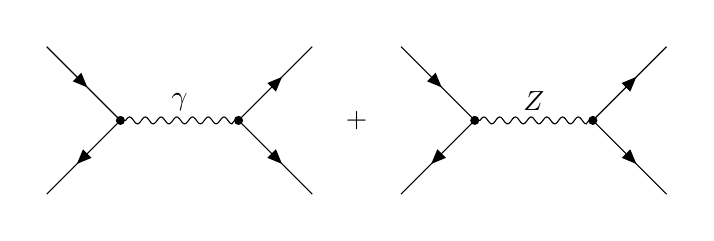
\begin{tikzpicture}
	\tikzfeynmanset{
		every vertex = {dot}
	}
	\begin{feynman}[small]
		\vertex (a1);
		\vertex[above left=1.5cm of a1] (a2) {};
		\vertex[below left=1.5cm of a1] (a3) {};
		\vertex[right = 1.5cm of a1] (a4);
		\vertex[above right=1.5cm of a4] (a5) {};
		\vertex[below right=1.5cm of a4] (a6) {};
		\vertex[right = 1.5cm of a4] (z) {+};
		\vertex[right = 1.5cm of z] (b1);
		\vertex[above left=1.5cm of b1] (b2) {};
		\vertex[below left=1.5cm of b1] (b3) {};
		\vertex[right = 1.5cm of b1] (b4);
		\vertex[above right=1.5cm of b4] (b5) {};
		\vertex[below right=1.5cm of b4] (b6) {};

		\diagram* {
			(a2) --[fermion] (a1) --[fermion] (a3),
			(a1) --[photon, edge label=\(\gamma\)] (a4) --[fermion] (a5),
			(a4) --[fermion] (a6),
			(b2) --[fermion] (b1) --[fermion] (b3),
			(b1) --[photon, edge label=\(Z\)] (b4) --[fermion] (b5),
			(b4) --[fermion] (b6),
		};
	\end{feynman}
	\end{tikzpicture}
\end{center}

The amplitude associated is
\begin{align*}
	\overline{|\mathcal{H}|}^2(s,t) = &\frac{2 e^{4} \left(t^2 + \left(s + t\right)^{2}\right)}{s^{2}}\\&
	+ \frac{4 e^{2} g_{4c}^{2} \left(1 - \frac{M_{z}^{2}}{s}\right) \left[t^{2} \left(\left(4 s_{W}^{2} - 1\right)^{2} - 1\right) + \left(s + t\right)^{2} \left(\left(4 s_{W}^{2} - 1\right)^{2} + 1\right)\right]}{M_{z}^{2} \Gamma_{z}^{2} + \left(s - M_{z}^{2}\right)^{2}}\\&
	+ \frac{2 g_{4c}^{4} \left[4\left(4 s_{W}^{2} - 1\right)^2\left(\left(s + t\right)^{2} - t^{2}\right) + \left(\left(s + t\right)^{2} + t^{2}\right) \left(\left(4 s_{W}^{2} - 1\right)^{2} + 1\right)^{2}\right]}{M_{z}^{2} \Gamma_{z}^{2} + \left(s - M_{z}^{2}\right)^{2}}
\end{align*}

The LP formula can be written as
\begin{equation}
	\overline{|\mathcal{A}^{LP}|}^2 = - \sum_{i, j} \eta_i \eta_j Q_i Q_j \frac{p_i \cdot p_j}{(p_i \cdot k)(p_j \cdot k)}\overline{|\mathcal{H}|}^2 = -C \overline{|\mathcal{H}|}^2
\end{equation}
And the NLP correction is
\begin{equation}
	\overline{|\mathcal{A}|}^2 = - \sum_{i, j} \xi_j\eta_i \eta_j Q_i Q_j \frac{p_{i\mu}}{(p_i \cdot k)} G_j^{\mu\nu}\pdv{\overline{|\mathcal{H}|}^2}{p_j^\nu}
\end{equation}
Since our expression for $\overline{|\mathcal{H}|}^2$ depends only on $s=(p_1+p_2)^2$ and $t=(p_1-p_3)^2$ the derivatives are
\begin{equation}
	\pdv{\overline{|\mathcal{H}|}^2}{p_1^\nu} = 2(p_1+p_2)_\nu\pdv{\overline{|\mathcal{H}|}^2}{s} + 2(p_1-p_3)_\nu\pdv{\overline{|\mathcal{H}|}^2}{t}
\end{equation}
\begin{equation}
	\pdv{\overline{|\mathcal{H}|}^2}{p_2^\nu} = 2(p_1+p_2)_\nu\pdv{\overline{|\mathcal{H}|}^2}{s}
\end{equation}
\begin{equation}
	\pdv{\overline{|\mathcal{H}|}^2}{p_3^\nu} = -2(p_1-p_3)_\nu\pdv{\overline{|\mathcal{H}|}^2}{t}
\end{equation}
\begin{equation}
	\pdv{\overline{|\mathcal{H}|}^2}{p_4^\nu} = 0
\end{equation}
\begin{align*}
	G_j^{\mu\nu}p_\nu &
	= \left(g^{\mu\nu} - \frac{p_j^\mu k^\nu}{p_j\cdot k}\right)p_\nu
	= \left(p^\mu - p_j^\mu\frac{p\cdot k}{p_j\cdot k}\right)
	= \frac{(p_j\cdot k)p^\mu - (p\cdot k)p_j^\mu}{p_j\cdot k}
\end{align*}
Simplifying the NLP expression;
\begin{alignat*}{3}
	\overline{|\mathcal{A}|}^2 &&
	= & - \xi_1\eta_1Q_1\sum_{i} \eta_i  Q_i  \frac{p_{i\mu}}{(p_i \cdot k)} G_1^{\mu\nu}\pdv{\overline{|\mathcal{H}|}^2}{p_1^\nu}
	- \xi_2\eta_2Q_2\sum_{i} \eta_i Q_i \frac{p_{i\mu}}{(p_i \cdot k)} G_2^{\mu\nu}\pdv{\overline{|\mathcal{H}|}^2}{p_2^\nu}\\&&&
	- \xi_3\eta_3Q_3\sum_{i} \eta_i Q_i \frac{p_{i\mu}}{(p_i \cdot k)} G_3^{\mu\nu}\pdv{\overline{|\mathcal{H}|}^2}{p_3^\nu}\\&&
	= & - 2\sum_{i} \eta_i Q_i \frac{p_{i\mu}}{(p_i \cdot k)}\left(\xi_1\eta_1Q_1\left(p_2^\mu - \frac{p_2 \cdot k}{p_1\cdot k}p_1^\mu\right)
	+\xi_2\eta_2Q_2 \left(p_1^\mu - \frac{p_1\cdot k}{p_2\cdot k}p_2^\mu\right)\right)\pdv{\overline{|\mathcal{H}|}^2}{s}\\&&&
	+ 2\sum_{i} \eta_i  Q_i  \frac{p_{i\mu}}{(p_i \cdot k)}\left(\xi_1\eta_1Q_1  \left(p_3^\mu - \frac{p_3 \cdot k}{p_1\cdot k}p_1^\mu\right)
	+\xi_3\eta_3Q_3 \left(p_1^\mu - p_3^\mu\frac{p_1\cdot k}{p_3\cdot k}\right)\right)\pdv{\overline{|\mathcal{H}|}^2}{t}\\&&
	= & - 2\left(\frac{\xi_1\eta_1Q_1}{p_1\cdot k}
	-\frac{\xi_2\eta_2Q_2}{p_2\cdot k} \right)\sum_{i} \eta_i Q_i \frac{(p_1\cdot k)(p_2\cdot p_i) - (p_2\cdot k)(p_1\cdot p_i)}{(p_i \cdot k)}\pdv{\overline{|\mathcal{H}|}^2}{s}\\&&&
	+ 2\left(\frac{\xi_1\eta_1Q_1}{p_1\cdot k} -\frac{\xi_3\eta_3Q_3}{p_3\cdot k}\right)\sum_{i} \eta_i  Q_i \frac{(p_1\cdot k)(p_3\cdot p_i) - (p_3\cdot k)(p_1\cdot p_i)}{(p_i \cdot k)}\pdv{\overline{|\mathcal{H}|}^2}{t}\\&&
	= & - 2\left(\frac{\eta_1Q_1}{p_1\cdot k}
	-\frac{\eta_2Q_2}{p_2\cdot k} \right)\left(\sum_{i} \eta_i Q_i \frac{(p_1\cdot k)(p_2\cdot p_i) - (p_2\cdot k)(p_1\cdot p_i)}{(p_i \cdot k)}\right)\pdv{\overline{|\mathcal{H}|}^2}{s}\\&&&
	+ 2\left(\frac{\eta_1Q_1}{p_1\cdot k} +\frac{\eta_3Q_3}{p_3\cdot k}\right)\left(\sum_{i} \eta_i  Q_i \frac{(p_1\cdot k)(p_3\cdot p_i) - (p_3\cdot k)(p_1\cdot p_i)}{(p_i \cdot k)}\right)\pdv{\overline{|\mathcal{H}|}^2}{t}
\end{alignat*}

\begin{align*}
	\frac{1}{4}\pdv{\overline{|\mathcal{H}|}^2}{s} = &\frac{M_{z}^{2} e^{2} g_{4c}^{2} \left(t^{2} \left(\left(4 s_{W}^{2} - 1\right)^{2} - 1\right) + \left(s + t\right)^{2} \left(\left(4 s_{W}^{2} - 1\right)^{2} + 1\right)\right)}{s^{2} \left(M_{z}^{2} \Gamma_{z}^{2} + \left(s - M_{z}^{2}\right)^{2}\right)}\\&
	+ \frac{e^{4} \left(s + t\right)}{s^{2}}
	- \frac{e^{4} \left(t^2 + \left(s + t\right)^{2}\right)}{s^{3}}\\&
	- \frac{2e^{2} g_{4c}^{2} s \left(1 - \frac{M_{z}^{2}}{s}\right)^2 \left(t^{2} \left(\left(4 s_{W}^{2} - 1\right)^{2} - 1\right) + \left(s + t\right)^{2} \left(\left(4 s_{W}^{2} - 1\right)^{2} + 1\right)\right)}{\left(M_{z}^{2} \Gamma_{z}^{2} + \left(s - M_{z}^{2}\right)^{2}\right)^{2}}\\&
	+ \frac{g_{4c}^{4} \cdot \left(M_{z}^{2} - s\right) \left(4s\left(4 s_{W}^{2} - 1\right)^2 \left(s+2t\right) + \left(t^{2} + \left(s + t\right)^{2}\right) \left(\left(4 s_{W}^{2} - 1\right)^{2} + 1\right)^{2}\right)}{\left(M_{z}^{2} \Gamma_{z}^{2} + \left(s - M_{z}^{2}\right)^{2}\right)^{2}}\\&
	+ \frac{2e^{2} g_{4c}^{2} \cdot \left(s + t\right) \left(1 - \frac{M_{z}^{2}}{s}\right) \left(\left(4 s_{W}^{2} - 1\right)^{2} + 1\right)}{M_{z}^{2} \Gamma_{z}^{2} + \left(s - M_{z}^{2}\right)^{2}}\\&
	+ \frac{g_{4c}^{4}(s+t) \left(4 \left(4 s_{W}^{2} - 1\right)^2 + \left(\left(4 s_{W}^{2} - 1\right)^{2} + 1\right)^{2}\right)}{M_{z}^{2} \Gamma_{z}^{2} + \left(s - M_{z}^{2}\right)^{2}}
\end{align*}

\begin{align*}
	\frac{1}{4}\pdv{\overline{|\mathcal{H}|}^2}{t} = &\frac{e^{4} \left(s + 2 t\right)}{s^{2}}
	+ \frac{2e^{2} g_{4c}^{2} \left(1 - \frac{M_{z}^{2}}{s}\right) \left((s+2t) \left(4 s_{W}^{2} - 1\right)^{2} + s\right)}{M_{z}^{2} \Gamma_{z}^{2} + \left(s - M_{z}^{2}\right)^{2}}\\&
	+ \frac{g_{4c}^{4} \cdot \left(4 s \left(4 s_{W}^{2} - 1\right)^2 + \left(s + 2t\right) \left(\left(4 s_{W}^{2} - 1\right)^{2} + 1\right)^{2}\right)}{M_{z}^{2} \Gamma_{z}^{2} + \left(s - M_{z}^{2}\right)^{2}}
\end{align*}

%\\
%For the simplest case of only two charged particles $Q_i=Q_j=e$, $\eta_1=-\eta_2$ we can compute the following factor;
%\begin{alignat*}{1}
%	\sum_{j}\eta_j \frac{(n_i\cdot k)(p_i\cdot p_j)-(p_i\cdot k)(n_i\cdot p_j)}{(p_j\cdot k)(p_i\cdot n_i)}
%	= -1-\frac{(n_1\cdot k)(p_1\cdot p_2)-(p_1\cdot k)(n_1\cdot p_2)}{(p_2\cdot k)(p_1\cdot n_1)}
%\end{alignat*}
%
%
%
%
%
%\begin{equation*}
%	2e^2\left(\frac{p_1}{p_1\cdot k}\Re{\mathcal{H}^*_{LO}J_{1} \mathcal{H}_{LO}}-\frac{p_2}{p_2\cdot k}\Re{\mathcal{H}^*_{LO}J_{1} \mathcal{H}_{LO}}-\frac{p_1}{p_1\cdot k}\Re{\mathcal{H}^*_{LO}J_{2} \mathcal{H}_{LO}}+\frac{p_2}{p_2\cdot k}\Re{\mathcal{H}^*_{LO}J_{2} \mathcal{H}_{LO}}\right)
%\end{equation*}
%\begin{align*}
%2e^2 \bigg(&\frac{1}{p_1\cdot k}\log(\frac{\bar{\mu}^2}{2p_1\cdot k})\bigg[
%2\left(\frac{p_2\cdot k}{p_1\cdot k}\frac{p_1^2}{p_1\cdot p_2}-\frac{p_2\cdot p_1}{p_1\cdot p_2}\right)
%+\frac{k\cdot p_1}{p_1\cdot k}\bigg]&\\&
%-\frac{1}{p_2\cdot k}\log(\frac{\bar{\mu}^2}{2p_1\cdot k})\bigg[
%2\left(\frac{p_2\cdot k}{p_1\cdot k}\frac{p_1\cdot p_2}{p_1\cdot p_2}-\frac{p_2^2}{p_1\cdot p_2}\right)
%+\frac{k\cdot p_2}{p_1\cdot k}\bigg]&\\&
%-\frac{1}{p_1\cdot k}\log(\frac{\bar{\mu}^2}{2p_2\cdot k})\bigg[
%2\left(\frac{p_1\cdot k}{p_2\cdot k}\frac{p_1\cdot p_2}{p_1\cdot p_2}-\frac{p_1^2}{p_1\cdot p_2}\right)
%+\frac{k\cdot p_1}{p_2\cdot k}\bigg]&\\&
%+\frac{1}{p_2\cdot k}\log(\frac{\bar{\mu}^2}{2p_2\cdot k})\bigg[
%2\left(\frac{p_1\cdot k}{p_2\cdot k}\frac{p_2^2}{p_1\cdot p_2}-\frac{p_1\cdot p_2}{p_1\cdot p_2}\right)
%+\frac{k\cdot p_2}{p_2\cdot k}\bigg]&\bigg)|\mathcal{H}_{LO}|^2
%\end{align*}
%\begin{align*}
%2e^2 \bigg(&\frac{1}{p_1\cdot k}\log(\frac{\bar{\mu}^2}{2p_1\cdot k})\bigg[
%-1	\bigg]&\\&
%-\frac{1}{p_2\cdot k}\log(\frac{\bar{\mu}^2}{2p_1\cdot k})\bigg[
%3\frac{p_2\cdot k}{p_1\cdot k}\bigg]&\\&
%-\frac{1}{p_1\cdot k}\log(\frac{\bar{\mu}^2}{2p_2\cdot k})\bigg[
%2\left(\frac{p_1\cdot k}{p_2\cdot k}\frac{p_1\cdot p_2}{p_1\cdot p_2}-\frac{p_1^2}{p_1\cdot p_2}\right)
%+\frac{k\cdot p_1}{p_2\cdot k}\bigg]&\\&
%+\frac{1}{p_2\cdot k}\log(\frac{\bar{\mu}^2}{2p_2\cdot k})\bigg[
%2\left(\frac{p_1\cdot k}{p_2\cdot k}\frac{p_2^2}{p_1\cdot p_2}-\frac{p_1\cdot p_2}{p_1\cdot p_2}\right)
%+\frac{k\cdot p_2}{p_2\cdot k}\bigg]&\bigg)|\mathcal{H}_{LO}|^2
%\end{align*}

\bibliographystyle{plain}
\bibliography{PhD_Bibliography.bib}

\end{document}
